% TODO Walk through all emails and see what people don't understand


\documentclass{article}

\usepackage[T1]{fontenc}
\usepackage{graphicx}
\usepackage{longtable}
\usepackage[colorlinks=true]{hyperref}
\usepackage[all]{xy}
\usepackage{nameref}
\usepackage{fullpage}
\usepackage{wrapfig}
\usepackage{array}

\begin{document}

\title{Timeplotters:\\
two tools for visualizing logs and temporal data}
\author{Eugene Kirpichov <ekirpichov@gmail.com>}
\date{\today}
\maketitle

\tableofcontents

\def\splot{\textbf{splot}}
\def\timeplot{\textbf{timeplot}}
\def\awk{\textbf{awk}}

\newcommand{\thumbnail}[1]{\includegraphics[width=0.12\textwidth]{#1}}

\newcommand{\inlinethumbnail}[1]{\framebox{$\vcenter{\hbox{\includegraphics[width=0.12\textwidth]{#1}}}$}}

\setlength{\parskip}{2mm plus1mm minus1mm}

\newcolumntype{V}{>{\centering\vspace{5px}\arraybackslash} m{.2\linewidth} }

\pagebreak
\section{Introduction}

\splot{} and \timeplot{} are tools for visualizing temporal data, especially useful for visualizing data from program logs.

You can get them and see the installation instructions at \url{http://jkff.info/software/timeplotters}. Both tools are heavily battle-tested and evolved in response to concrete visualization requirements at a large-scale cluster computing project which the author was part of, though the tools are in no way bound to this particular domain.

\begin{wrapfigure}[4]{r}{120pt}
\vspace{-25pt}
\center
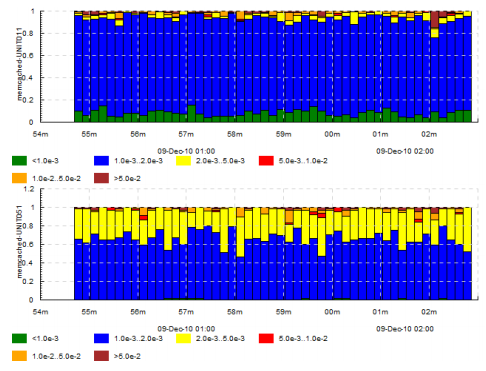
\includegraphics[height=60pt]{pics/tplot/tplot-motivating-example.png}
\end{wrapfigure}
  
\timeplot{} draws quantitative graphs about several streams of events happening over time, e.g. you can use it to compare the distribution of database access latencies from two machines; to draw the number of requests being concurrently processed by each server at each moment, etc.

\begin{wrapfigure}[7]{r}{120pt}
\vspace{-5pt}
\center
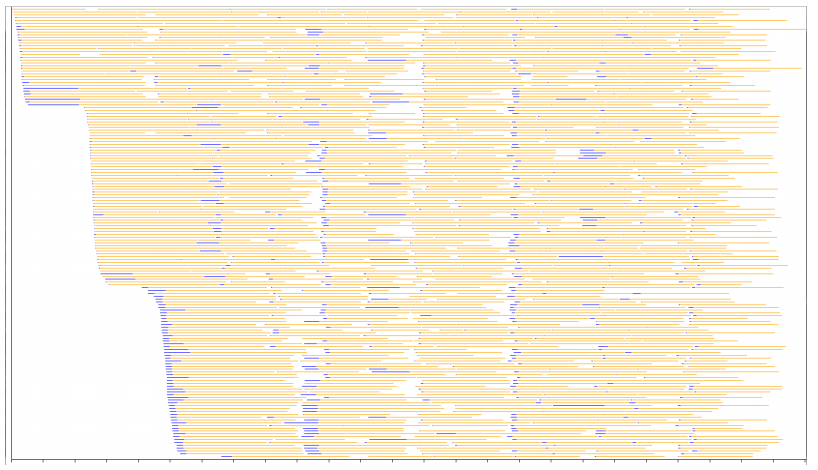
\includegraphics[height=60pt]{pics/splot/splot-main-example.png}
\end{wrapfigure}
\splot{} draws a single Gantt-like chart with a birds-eye view of the activity of a number of concurrent processes, color-coding the state of each process at each moment (e.g. processing one of several jobs, or being in a particular stage of processing). This allows to see peculiar system-level behavior patterns and usually allows to instantly isolate system-level performance bottlenecks which very often show themselves as distinct visual patterns. Section \nameref{sec:splot-motivation} gives an example of what non-trivial aspects of a program's behavior \splot{} can show.

\textbf{These characteristics} make the tools useful for exploratory analysis:

\begin{itemize}
\item \textbf{Input is trivial to generate} from raw logs by usual text processing tools such as awk or perl
\item You can generate \textbf{different plots from the same input}
\item Fast enough to draw \textbf{many millions of events} in tens of seconds, potentially unlimited input size
\item Tools are invoked by \textbf{one-liners}
\end{itemize} 

Both \timeplot{} and \splot{} accept input in a strictly specified format, not arbitrary logs. A file in this format is called \emph{trace}. However, this format is designed to be trivial to generate from log files, e.g. using text processing tools such as awk, sed or perl. I use \awk{}, it shines at one-liners (google ``awk one-liners'').

The general pattern of usage is displayed on figure \ref{fig:general-usage}: you use an awk one-liner to generate the \emph{trace} and invoke the tool on it.

\begin{figure}[t]
\center
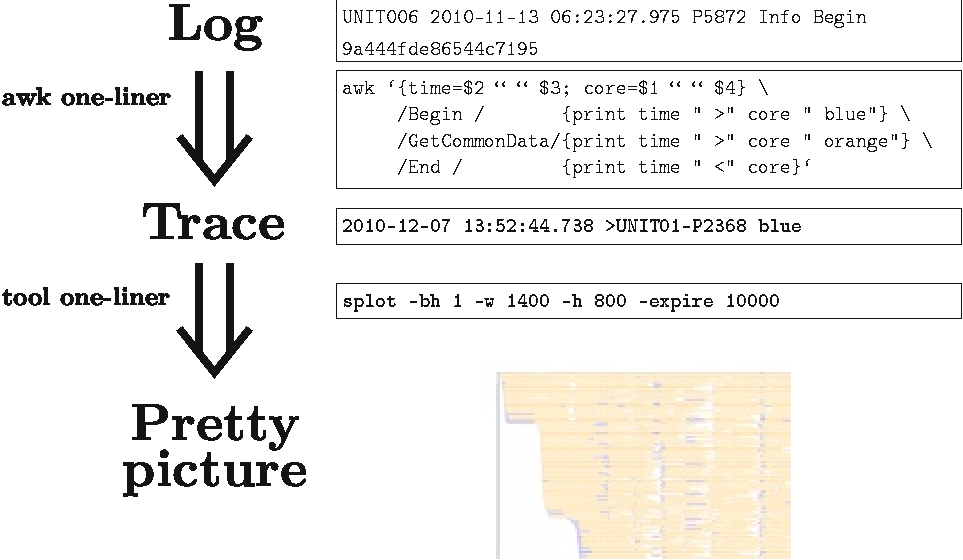
\includegraphics[width=0.6\textwidth]{general-usage.pdf}
\caption{The general pattern of usage of both \timeplot{} and \splot{}.}
\label{fig:general-usage}
\end{figure}

\begin{verbatim}
$ awk '/some log entry/{emit an event into trace} \
       /another log entry/{emit another event...}' \
       log.txt > trace.txt
$ splot -if trace.txt -o picture.png ..options..
\end{verbatim}

\textbf{Let us look at a real-life example} without considering it in too much detail. Use it only for the purpose of understanding the general pattern of usage.
\pagebreak

% TODO Maybe use memcached example here instead?

In this example, we're drawing the activity of a computational cluster using \splot{}. There's a bunch of worker processes which process tasks from a shared queue. Every task has two stages: 1) fetch data from memcached and 2) run computations. \textbf{Here we'll just show how to run the tool, and not explain what the parameters or even the result mean.}

The log entries look like this:

\begin{tabular}{llllll}
\emph{Machine} & \emph{Date/time} & \emph{Process ID} & \emph{Level} & \emph{Operation} & \emph{Task ID} \\
\footnotesize{\texttt{UNIT011}} & \footnotesize{\texttt{2010-12-09 01:54:41.853}} & \footnotesize{\texttt{P3964}} & \footnotesize{\texttt{Debug}} & \footnotesize{\texttt{GetCommonData}} & \footnotesize{\texttt{390256d1/49}} \\
\end{tabular}

Operation can be one of \verb|Begin| (starting a task), \verb|GetCommonData| (finished getting task data from database, starting computations), \verb|End| (computations for a task finished).

\begin{verbatim}
$ awk '{time=$2 " " $3; core=$1 " " $4} \
       /Begin /       {print time " >" core " blue"} \
       /GetCommonData/{print time " >" core " orange"} \
       /End /         {print time " <" core}' log.txt > trace.txt
$ splot -if trace.txt -o splot.png -bh 1 -w 1400 -h 800 -expire 10000
\end{verbatim}

\centerline{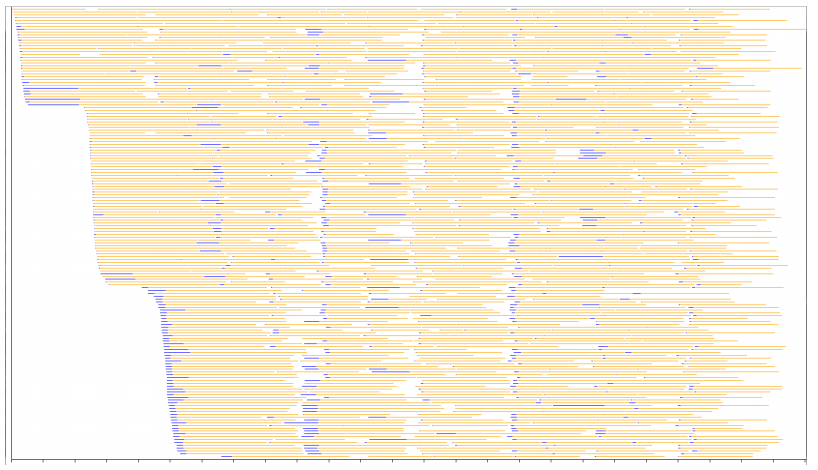
\includegraphics[width=0.8\textwidth]{pics/splot/splot-main-example.png}}

You can see that it took just 2 commands to produce a picture.

The picture is actually very interesting and highlights many performance problems in the original program. The curious reader is advised to look at section \nameref{sec:splot-motivation} where we discuss this case in detail.

Now let's consider the tools in detail.

\pagebreak
\section{\timeplot{}~--- drawing quantitative plots from event streams}
\label{sec:tplot-intro}

\timeplot{} allows you to visualize temporal data in different ways, with the intention to help you spot patterns. It takes as input a sequence of events in a fixed format (there are several types of events), and draws the quantitative characteristics of that sequence in many different ways~--- e.g. you can \textbf{compare the frequency} of different types of events per time unit, or to look at the distribution of \textbf{event durations}, etc.

\textbf{The input} to \timeplot{} is a sequence of events of the form ``event X happened'', ``interval event X started/finished'', ``a numeric or discrete variable P took value X''. Every event happens on a particular \emph{input track} and at a particular time. The types of events are specified in section \nameref{sec:tplot-input-format}. Different types of events can be used with different types of visualizations.

\textbf{The output} is a vertical stack of plots with a common time axis. Each plot corresponds to one \emph{output track}. Usually \emph{input tracks} correspond to output tracks 1-to-1, but sometimes the relation is more complex (multiple tracks on 1 plot, or 1 track on multiple plots)~--- see \nameref{sec:tplot-concepts}. Every output plot is one of several types (e.g. simple dot plot, line plot, quantile plot, etc.). The kind of plot to draw on a particular output track is specified by the \emph{plot kind mapping}, also described in section \nameref{sec:tplot-concepts}.

An example result of \timeplot{} is shown on figure \ref{fig:tplot-example}.

\begin{figure}[h]
\center
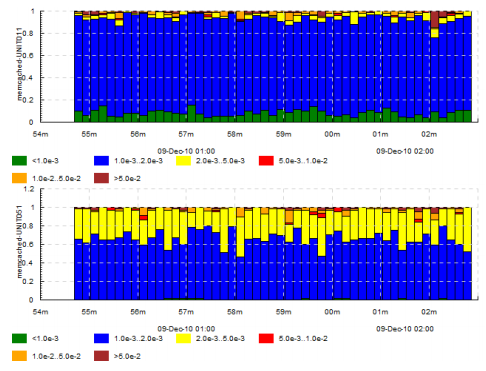
\includegraphics[width=0.6\textwidth]{pics/tplot/tplot-motivating-example.png}
\caption{\timeplot{} example: distribution of memcached access latencies from the same rack and from a different rack. Built from a log that had lines about starts and completions of requests to memcached.}
\label{fig:tplot-example}
\end{figure}

\pagebreak
\subsection{Simple example}
\label{sec:tplot-simple-example}
This section considers in detail the simplest and most intuitive example possible: a dot plot of a single time-varying value.

Assume that we have a program that sometimes does requests to a database server (``Arcadia''~--- this is a real-life example from Yandex, and Arcadia is the codename of its core search engine) and logs their durations:

\begin{verbatim}
...
2010-05-11 18:25:05.435 Arcadia request took 820 ms
...
\end{verbatim}

We're interested in looking at the structure of these durations and its change over time. A simple dot plot is a perfect starting point.

First, \textbf{generate the trace}: for each line of interest in the log, we need to emit a corresponding \emph{numeric measurement} event into the trace (see reference on event types in section \nameref{sec:tplot-concepts} and on their textual format in section \nameref{sec:tplot-input-format}).

The trace should look like this:
\begin{verbatim}
...
2010-05-11 18:25:05.435 =arc 820
...
\end{verbatim}

This is trivial to achieve with an awk one-liner:
\begin{verbatim}
$ awk '/Arcadia req/{print $1 " " $2 " =arc " $6}' log.txt > trace.txt
\end{verbatim}

Now we can \textbf{generate the plot}: we need to tell \timeplot{} the input and output filenames and what kind of chart to draw.
\begin{verbatim}
$ tplot -if trace.txt -o arc.png -dk dots
\end{verbatim}

The parameter \verb|-dk| means ``default chart kind'': just draw all tracks (in this case the only track) using this kind of chart (\verb|dots|). So, the track mapping process is involved here in the most trivial form (see section \nameref{sec:tplot-track-mapping} for less trivial forms).

\begin{wrapfigure}[2]{c}{50pt}
\vspace{-25pt}
\center
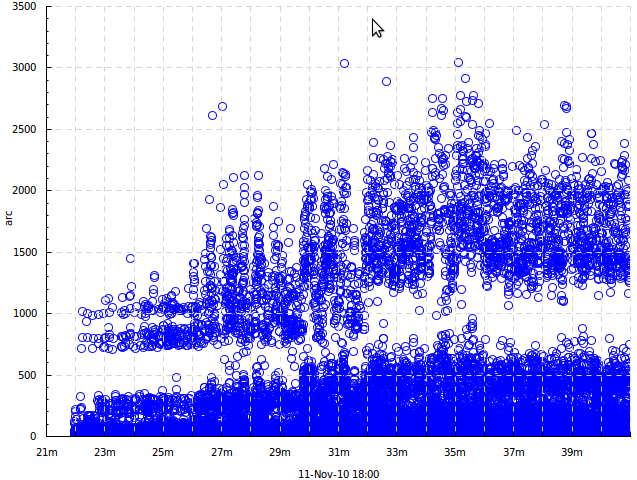
\includegraphics[height=40pt]{pics/tplot/dots.png}
\end{wrapfigure}
And we get figure \ref{fig:tplot-simple-example} (next page).

\begin{figure}[h!]
\center
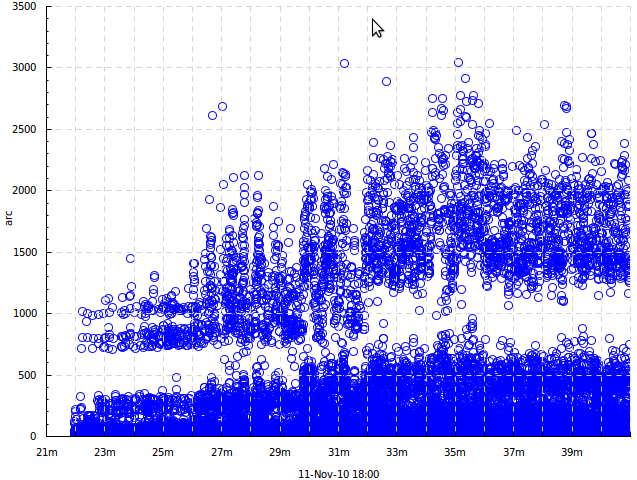
\includegraphics[width=0.6\textwidth]{pics/tplot/dots.png}
\caption{Simple example of \timeplot{}~--- a dot plot of a single variable}
\label{fig:tplot-simple-example}
\end{figure}

We see the following features:
\begin{itemize}
\item The times clearly split into higher and lower values, obviously corresponding to cache hits and cache misses within Arcadia.
\item At some point the distribution suddenly changes to the worse and requests start taking more time. I do not remember what was the reason for that, but there certainly was one.
\item There's a lot of overplotting on the picture; it's difficult to understand the distribution more precisely. To do that, we'll need quantile plots or bin plots (see section \nameref{sec:tplot-plot-kinds}). An alternative is to use semi-transparent dots (e.g. \verb|-dk 'dots 0.3'| would give 30\% opacity). There exist other ways of coping with overplotting (just google \emph{overplotting}), but they're not currently implemented in \timeplot{}.
\end{itemize}

\textbf{Where to go next:}

From this simple example you can go several ways:
\begin{itemize}
\item Get a glimpse of the power of \timeplot{} in a more serious example~--- continue to section \nameref{sec:tplot-motivation} where a reasonably complex real-world example is considered.
\item Explore the ways to \textbf{map event streams onto charts}: draw multiple tracks, display a single input data point on multiple charts or vice versa, display data points from multiple tracks on a single plot (e.g. a color-coded dot plot)~--- see section \nameref{sec:tplot-track-mapping}.
\item Learn to use the \textbf{more complex event types} (e.g. discrete, impulse, edge and interval events) and to draw other types of charts on them~--- read section \nameref{sec:tplot-concepts} and continue to section \nameref{sec:tplot-plot-kinds}.
\item Draw more interesting \textbf{types of charts}~--- just go to section \nameref{sec:tplot-plot-kinds}.
\item Take a look at the \textbf{example charts gallery} and choose something that looks interesting or applicable to your case~--- go to section \nameref{sec:tplot-gallery}.
\end{itemize}

\subsection{Motivation: More complex example}
\label{sec:tplot-motivation}
In this section we'll show a moderately complex real-world example of usage of \timeplot{}, with the goal to show its power and inspire the reader to learn more, but without the goal to provide detailed explanations. To become capable of using \timeplot{} for similar purposes \emph{yourself}, you'll have to actually read the next chapters.

Consider the log format described in the \nameref{sec:tplot-intro}~--- the one where tasks consist of a ``fetching data from memcached'' stage and ``computational'' stage, delimited by \verb|Begin|, \verb|GetCommonData|, \verb|End|.

Suppose that we have several racks of servers and just one memcached server. Let us compare how memcached latencies differ when it is accessed by workers from different racks (since cross-rack access requires an extra network packet hop through a switch device, accesing from the same rack should be faster).

memcached is on rack 1. Let us specifically compare performance on machines \verb|UNIT011| and \verb|UNIT051|. So, we should expect access from \verb|UNIT011| to be faster.

The filtered log looks like this:
\begin{verbatim}
...
UNIT011 2010-12-09 01:54:41.853 P3964 Debug GetCommonData 390256d1/49
UNIT011 2010-12-09 01:54:41.927 P3964  Info Begin 390256d1/51
UNIT011 2010-12-09 01:54:41.928 P3964 Debug GetCommonData 390256d1/51
UNIT051 2010-12-09 01:54:42.045 P3832  Info Begin 390256d1/99
UNIT051 2010-12-09 01:54:42.045 P3164  Info Begin 390256d1/98
UNIT051 2010-12-09 01:54:42.046 P3164 Debug GetCommonData 390256d1/98
...
\end{verbatim}

Let us make this into a trace file for \timeplot{}:
\begin{verbatim}
$ awk '{t=$2 " " $3; p="memcached-" $1 "." $4}
       /Begin /        {print t " >" p} 
       /GetCommonData /{print t " <" p}'
       log.txt > trace.txt
\end{verbatim}

The trace will look like this:
\begin{verbatim}
...
2010-12-09 01:54:41.853 <memcached-UNIT011.P3964
2010-12-09 01:54:41.927 >memcached-UNIT011.P3964
2010-12-09 01:54:41.928 <memcached-UNIT011.P3964
2010-12-09 01:54:42.045 >memcached-UNIT051.P3832
2010-12-09 01:54:42.045 >memcached-UNIT051.P3164
2010-12-09 01:54:42.046 <memcached-UNIT051.P3164
...
\end{verbatim}

Here the ``track names'' correspond to different processes (though in general, as we'll see later, track names have broader meaning in \timeplot{}), \verb|>| means the beginning of an activity and \verb|<| means the end (these are two of the different event types).

Now we'll plot the distribution of durations of memcached access times according to these \verb|>| and \verb|<| events.

\begin{verbatim}
$ tplot -if trace.txt -o latencies.png
        -dk 'within[-] duration binf 10 0.001,0.002,0.005,0.01,0.05'
\end{verbatim}

\begin{wrapfigure}[3]{c}{70pt}
\vspace{-25pt}
\center
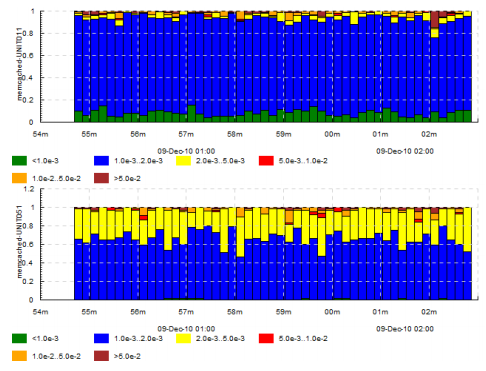
\includegraphics[height=50pt]{pics/tplot/tplot-motivating-example.png}
\end{wrapfigure}

For now do not concern yourself with the meaning of the value of the \verb|-dk| parameter, it will be explained later (in section \nameref{sec:tplot-plot-kinds}). Just concentrate on the input (how easy it is to generate from the logs) and the output (how much it tells about the system). The result is shown on figure \ref{fig:tplot-motivating-example} (next page).

\pagebreak

\begin{figure}[h]
\center
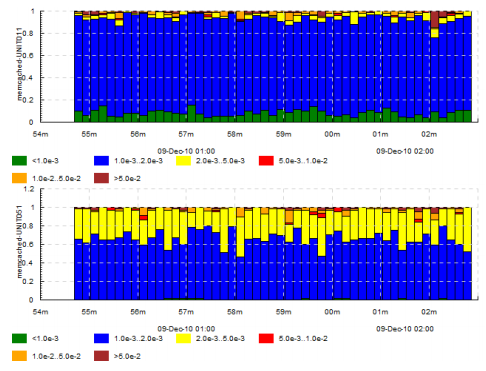
\includegraphics[width=0.8\textwidth]{pics/tplot/tplot-motivating-example.png}
\caption{\timeplot{} example: distribution of memcached access latencies from the same rack and from a different rack.}
\label{fig:tplot-motivating-example}
\end{figure}

\textbf{Explanation of the output:} The graph above corresponds to access from \verb|UNIT011|, below from \verb|UNIT051|. Both graphs have time on the X axis and latency on the Y axis. Time is cut into 10-second bins represented by a stack of colored bars. Within each stack (see legend and compare to the invocation of \verb|tplot| above):
\begin{itemize}
\item Height of the green bar shows the fraction of latencies under 0.001s
\item Height of the blue bar shows the fraction of latencies in 0.001s--0.002s
\item Height of the yellow bar shows the fraction of latencies in 0.002s--0.005s
\item Height of the red bar shows the fraction of latencies in 0.005s--0.01s
\item Height of the orange bar shows the fraction of latencies in 0.01s--0.05s
\item Height of the brown bar shows the fraction of latencies above 0.05s
\end{itemize}

Together these fractions add up to 1.

\textbf{The graphs differ}:
\begin{itemize}
\item There are \textbf{no green bars} on the second graph, i.e. access from a different rack is never under 0.001s
\item The \textbf{yellow bars are a lot larger} on the second graph, i.e. times in 0.002s--0.005s are much more frequent when accessing from a different rack
\end{itemize}

\textbf{To reiterate:} given the log, the following commands:

\begin{verbatim}
$ awk '{t=$2 " " $3; p="memcached-" $1 "." $4}
       /Begin /        {print t " >" p} 
       /GetCommonData /{print t " <" p}'
       log.txt > trace.txt
$ tplot -if trace.txt -o latencies.png
        -dk 'within[-] duration binf 10 0.001,0.002,0.005,0.01,0.05'
\end{verbatim}

\ldots give us figure \ref{fig:tplot-motivating-example} which shows how exactly the distributions of access latencies from different racks differ and emphasize the importance of choosing a nearby memcached according to network topology.

This example illustrated the mode of usage of \timeplot{}, the ease of generating input for it from an arbitrary log and the terseness of its syntax for specifying the kind of graph to be plotted. We'll now give some basic definitions and then proceed to a formal and exhaustive reference.

\subsection{Concepts}
\label{sec:tplot-concepts}

This section lists the concepts necessary for precisely understanding the rest of the manual. You can quickly skim over them now just to get a feeling of what they're about, and return to them later when something is unclear.

\begin{description}
\item[Event] The atomic unit of information in the input trace. It can be one of several types: ``something has happened'' (this is called an \emph{impulse event}), ``something has started/finished'' (this is called an \emph{edge event}, and the activity delimited by start/finish is called an \emph{interval event}), ``some magnitude had a particular value'' (\emph{measurement event}) etc. The types of events correspond to what is usually found in typical program log entries, so they're very easy to generate from logs. Every event happens on a particular \emph{input track} and at a particular time, for example: \verb|2012-06-04 14:24:05.384 =rtime.mcd1 5.371|, this is a numeric measurement event (``\texttt{=}''), here \verb|rtime.mcd1| is the input track name and \verb|2012-06-04 14:24:05.384| is the timestamp.
\item[Input track] A named group of events in the \emph{input trace}. Usually corresponds to a single magnitude being measured or to a single family of activities, e.g. there could be an input track for request execution times named ``rtime'' or a track for types of received messages by client C1 named ``mtype-C1''. Thus, an input track nearly always consists of events of the same type. Here we would have the input trace consist of numeric measurement events with track ``rtime'' (see different types of events described in section \nameref{sec:tplot-input-format}).
\item[Output track] A named group of events in the \emph{output plots}. The output track of an event is often equal to its input track, but in general it is determined from its input track by the process of \emph{track mapping} described in section \nameref{sec:tplot-track-mapping}. All events with the same output track are shown on the same output plot.
\item[Output plot] A single plot in the resulting picture. The picture consists of several output plots vertically stacked together with a common time axis. A single output plot is based on values from a single output track, which may have events from one or more input tracks.
\item[Track mapping] The process by which events from different input tracks are mapped onto output tracks, e.g. to make events from multiple input tracks participate in a single output plot, or to make events from a single input track participate in multiple output plots. It is controlled, together with \emph{plot kind mapping}, by \verb|+k|, \verb|-k|, \verb|+dk|, \verb|-dk| options and by the \verb|within[SEP]| plot kind. The process is described in section \nameref{sec:tplot-track-mapping}.
\item[Plot kind] The type of an output plot: e.g. dot plot, line plot, quantile plot etc. There are also a couple of ``meta'' plot kinds: duration plots and ``within''-plots. Plot kinds usually have parameters, e.g. the percentiles of interest on a quantile plot. Plot kinds are described in section \nameref{sec:tplot-plot-kinds}.
\item[Plot kind mapping] The process by which we determine what plot kind to use for visualizing a particular output track. It also depends on \verb|+k|, \verb|-k|, \verb|+dk| and \verb|-dk| options, happens together with \emph{track mapping} and is described in detail in section \nameref{sec:tplot-track-mapping}.
\end{description}

To put it together: Input events belong to input tracks and get mapped onto output tracks via track mapping. Every output track gives rise to an output plot, its kind determined by plot kind mapping. Output plots are stacked vertically with a common time axis.

The following concepts are important for understanding the different event types and some plots produced from them:
\begin{description}
\item[Measurement event] An event that denotes that a particular parameter was measured to have a particular value (e.g.: the amount of free memory was measured to be 2.5Gb), or that something happened with a particular value of a parameter. E.g.: an I/O write request \emph{for 65536 bytes} arrived (e.g. \verb|... =writeBytes 65536|)~--- a numeric measurement; or an I/O request \emph{of type ``write''} has arrived (e.g. \verb|... =requestType `WRITE|)~--- a discrete measurement.
\item[Impulse event] An input event without parameters that just denotes that something has happened, determined solely by its input track. E.g. if you're interested in the number of completed requests per second (e.g. \verb|... !requestCompleted|), you can have an input trace with impulse events on the track \verb|requestCompleted| and draw an ``activity count'' plot of that (\verb|acount|).
\item[Edge event (counter bump)] An input event without parameters that denotes that some activity (interval event) has \emph{started} or \emph{finished}. It can at the same time be thought of as a bump of +1 (\verb|>request|) or -1 (\verb|<request|) of the logical counter associated with this event's input track.
\item[Counter] A logical time-varying variable associated with an \emph{input track} which can be bumped by start/finish (\emph{edge}) events. E.g. if your input trace includes events like ``started/finished executing a request'' (e.g. \verb|... >request|, \verb|<request|), then \timeplot{} will keep a logical counter that can be used to plot the number of concurrently executing requests.
\item[Interval event] The logical activity delimited by a start and finish event. More precisely, the period during which a \emph{counter} is greater than zero. The duration of interval events can be measured (producing a bunch of numeric measurement events) and you can draw all kinds of plots about these numeric events, e.g. if your input trace has ``request started/request finished'' events but doesn't have numeric events about request durations, you can still draw a quantile plot of request durations. This is called a \emph{duration plot}.
\item[Duration plot] A meta-plot which means ``plot something else, using as input the durations of interval events formed by edge events of this track'' (e.g. \verb|duration quantile 1 0.5,0.75,0.95|).
\end{description}

We advise you to revisit section \nameref{sec:tplot-motivation} and see if you now better understand the concepts involved there.

\pagebreak
\subsection{Input format}
\label{sec:tplot-input-format}

The general format of a \timeplot{} event is as follows:
\begin{verbatim}
TIMESTAMP [!<>=@]TRACK [VALUE]
\end{verbatim}

For example:
\begin{verbatim}
2012-06-04 14:24:13.389 !requestCompleted
2012-06-04 14:24:13.389 !userLogIn Joe
2012-06-04 14:24:13.389 >request.mcd1
2012-06-04 14:24:13.389 <request.mcd1
2012-06-04 14:24:13.389 =rtime 37.2
2012-06-04 14:24:13.389 =cache `MISS
2012-06-04 14:24:13.389 @phase blue
\end{verbatim}

The table below explains the meaning of all the event types.

\begin{tabular}{|l|p{200px}|l|}
\hline
Syntax & Meaning & Example \\
\hline
\verb|!TRACK| & Impulse event. & \verb|!requestCompleted| \\
\hline
\verb|!TRACK TEXT| & Impulse event with a text label. & \verb|!userLogIn Joe| \\
\hline
\verb|>TRACK| & Interval event start / counter bump +1. & \verb|>requestCompleted| \\
\hline
\verb|<TRACK| & Interval event finish / counter bump -1. & \verb|<requestCompleted| \\
\hline
\verb|=TRACK NUMBER| & Numeric measurement event. & \verb|=rtime 37.2| \\
\hline
\verb|=TRACK `TEXT| & Discrete measurement event. & \verb|=cache `MISS| \\
\hline
\verb|@TRACK COLOR| & Colored interval event start. & \verb|@phase blue| \\
\hline
\end{tabular}

\pagebreak
\subsection{Plot kinds}
\label{sec:tplot-plot-kinds}
This section describes all the chart kinds supported by \timeplot{} and gives recommendations on their usage.

Remember that the input data for each chart is events with a common \emph{output track} (see section \nameref{sec:tplot-track-mapping}), i.e. possibly events from multiple \emph{input tracks}.

Many of the chart kinds accept a ``bin width'' parameter: for example, \texttt{quantile 10 0.5,0.9,0.95} has a bin width of 10 seconds. This means that \timeplot{} will slice the time axis into 10-second bins, compute the 50\%, 90\% and 95\% quantiles of data in each bin and visualize the result in some way.

\subsubsection{Special kinds}
\noindent
\textbf{Empty chart~--- \texttt{none}}. This means ``do not draw this output track at all''. This is useful if you have prepared a trace from a large log file and invoke \timeplot{} several times on it, omitting some tracks altogether.

\noindent
\textbf{Chart over interval durations~--- \texttt{duration XXX} or \texttt{duration drop XXX}}. This means ``draw chart of kind XXX over the numeric durations of interval events delimited by start/finish events (``\verb|>|''/``\verb|<|'') on this track'' (see section \nameref{sec:tplot-concepts}). Durations are measured in seconds. If \verb|drop| is specified, then names of the original input tracks are replaced by the name of the output track (of course, this only makes a difference if multiple input tracks map to this output track).

For example, suppose you're measuring \textbf{processing of requests by several stages} of a single-threaded pipeline (i.e., every stage of the pipeline processes at most 1 item at a time). Then your log might say:
\begin{verbatim}
.... >process.stage1
.... >process.stage2
.... <process.stage1
.... >process.stage3
.... >process.stage1
.... <process.stage2
....
\end{verbatim}

If you're interested in making a dot plot of processing durations by different stages of the pipeline, you might want to do it in two ways:
\begin{itemize}
 \item 1 plot per stage: just use \texttt{-dk 'duration dots'}.
 \item 1 plot combined, with dots colored according to stage: use \verb|-dk 'within[.] duration dots'|. Then all these tracks will be put onto the same otput track \verb|process|, but their original names will be preserved and you'll get a plot like this: \inlinethumbnail{pics/tplot/thedeemon-dots-all.png}.
 \item If you use \verb|-dk 'within[.] duration drop dots'|, you'll get this: \inlinethumbnail{pics/tplot/thedeemon-dots-drop.png}, but this is likely not what you wanted.
\end{itemize}

On the other hand, suppose you're measuring the durations of \textbf{processing of requests themselves}. Then your log might say:
\begin{verbatim}
.... >process.14ca3ef7
.... <process.a28f3b13
....
\end{verbatim}

In this hypothetical log, all request ids are unique (contrary to pipeline stage names in the previous example). So, if we try drawing a dot plot of their durations using \verb|-dk 'within[.] duration dots'|, we'll get a plot where every dot has a different color, which makes no sense (and is not even processible at all by plot types such as \verb|quantile|). That's what \verb|duration drop XXX| is for: we can use \verb|-dk 'within[.] duration drop dots'| and the output track \verb|process| will contain durations of the requests with input track names not like \verb|process.14ca3ef7|, but simply \verb|process|, drawn in a single color.

\noindent
\textbf{Chart for M:1 track mapping~--- \texttt{within}}. This is not a chart kind proper, it's a means for displaying values from multiple input tracks on a single chart. See section \nameref{sec:tplot-track-mapping}.

% TODO Complex example

\pagebreak
\subsubsection{Kinds for numeric data}
All the following chart kinds work on numeric measurement events, i.e. events of the form \texttt{.... =TRACK VALUE}, e.g. \texttt{2012-08-07 18:04:35 =rtime 52.1}.

\noindent
\textbf{Simple dot plot~--- \texttt{dots [ALPHA]}}. When multiple input tracks map to this output track, the different input tracks are drawn with different colors. \texttt{ALPHA} is an optional opaqueness level: 0 means completely transparent, 1 means completely opaque. This helps to deal with overplotting, when there are too many values to display.

Example with 1 input track (\texttt{dots} without alpha):

\centerline{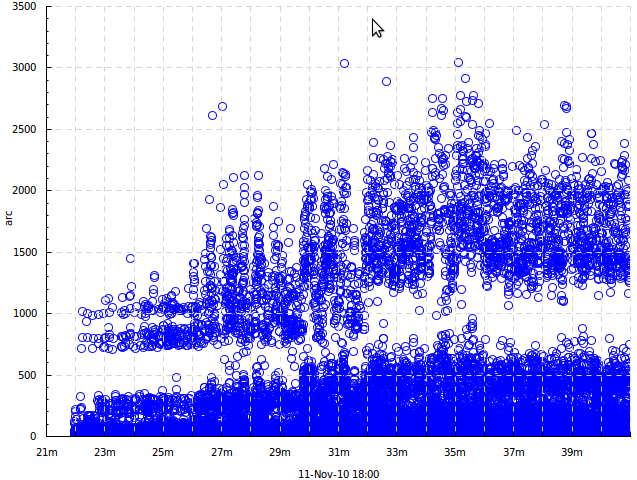
\includegraphics[width=0.5\textwidth]{pics/tplot/dots.png}}

This is the same graph as in section \nameref{sec:tplot-simple-example}: response times of a search engine server are drawn.
% TODO Make "Example xxx: [image]" non-page-broken.
Example with multiple input tracks (\texttt{dots} without alpha):

\centerline{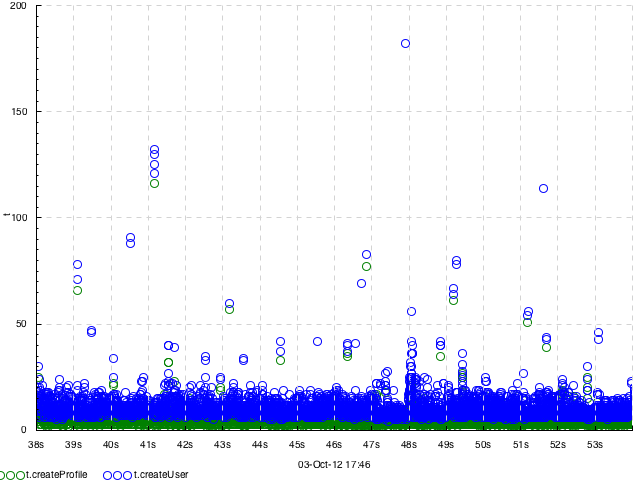
\includegraphics[width=0.5\textwidth]{pics/tplot/dots-create-user-and-profile.png}}

Previous example with \texttt{dots 0.2}:

\centerline{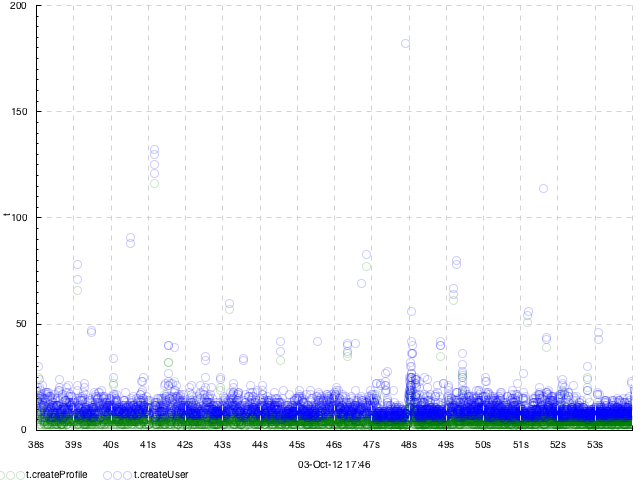
\includegraphics[width=0.5\textwidth]{pics/tplot/dots-create-user-and-profile-alpha.png}}

\pagebreak
\noindent
\textbf{Simple connected line plot~--- \texttt{lines}}. Same as \texttt{dots}, but the dots are connected. When multiple input tracks map to this output track, the different input tracks are drawn with different colors.

Example with 1 input track per output track:

\centerline{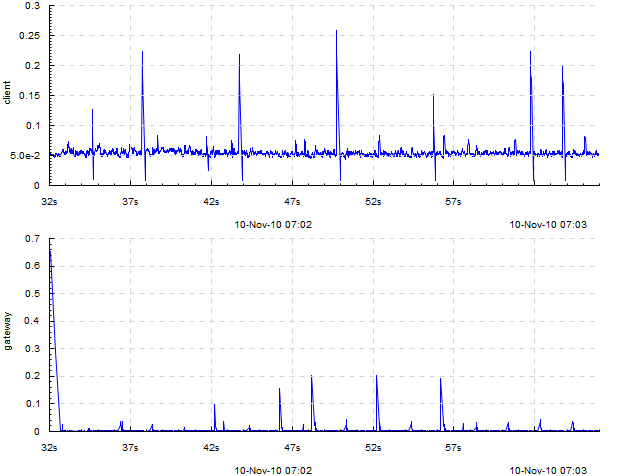
\includegraphics[width=0.8\textwidth]{pics/tplot/lines.png}}

These are request execution times as seen by 1) the caller (\emph{client}) and 2) the callee (\emph{gateway}), plotted from a trace with events of the form \texttt{=client 0.053}.

\pagebreak
\noindent
\textbf{Line plot of binned sum~--- \texttt{sum N [TYPE]}}~--- slice time axis into N-second bins; draw a simple line plot of sums of values in each bin. When multiple input tracks map to this output track, the different input tracks are drawn with different colors. If TYPE is \texttt{overlayed}, subplots for different input tracks are just overlayed on each other. If TYPE is \texttt{stacked} (default), they are ``accumulated'' so you can see how the total sum adds up from them. This is useful to understand, e.g., how big is the role of a step of some computation in the total time it takes. If the number of values per bin is usually the same, then \texttt{sum} also gives an impression of the average value\footnote{It's probably worth implementing an actual \texttt{avg} chart kind.}.

Example with two tracks, on the same data as in \texttt{dots}: \texttt{sum 1 overlayed}

\centerline{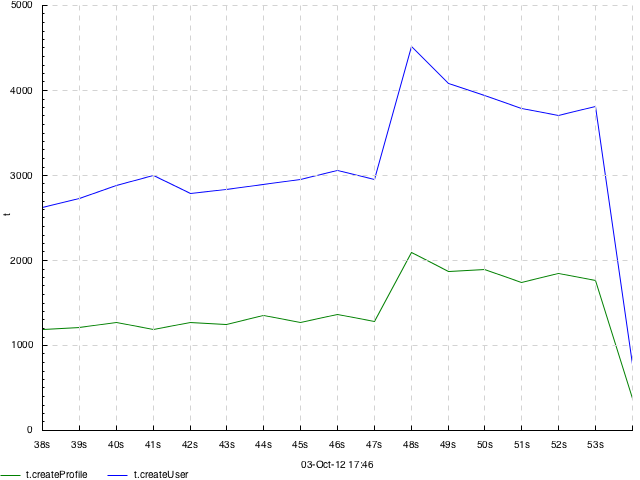
\includegraphics[width=0.5\textwidth]{pics/tplot/sum-create-user-and-profile-overlayed.png}}

Same with \texttt{sum 1 stacked} or just \texttt{sum 1}:

\centerline{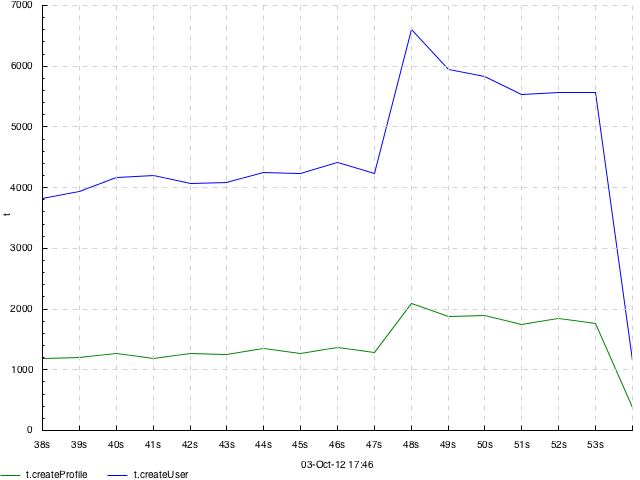
\includegraphics[width=0.5\textwidth]{pics/tplot/sum-create-user-and-profile-stacked.png}}

\pagebreak
\noindent
\textbf{Line plot of cumulative sum~--- \texttt{cumsum N [TYPE]}}~--- same as \texttt{sum}, but accumulation happens not in every bin but from the beginning of time.
Example with two tracks, on the same data as in \texttt{dots}: \texttt{cumsum 1 overlayed}

\centerline{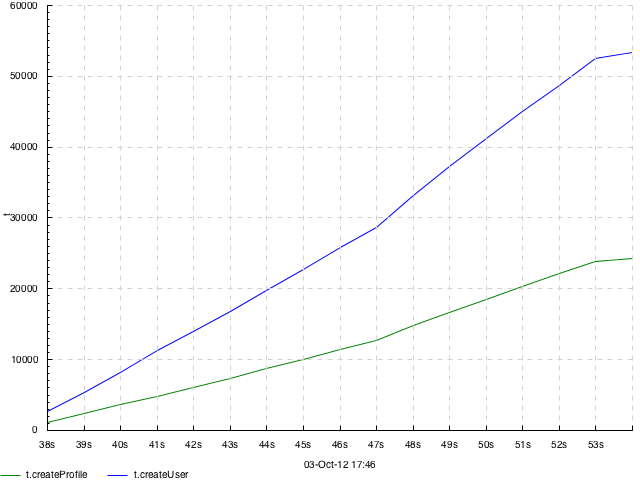
\includegraphics[width=0.5\textwidth]{pics/tplot/cumsum-create-user-and-profile-overlayed.png}}

Same with \texttt{cumsum 1 stacked} or just \texttt{cumsum 1}:

\centerline{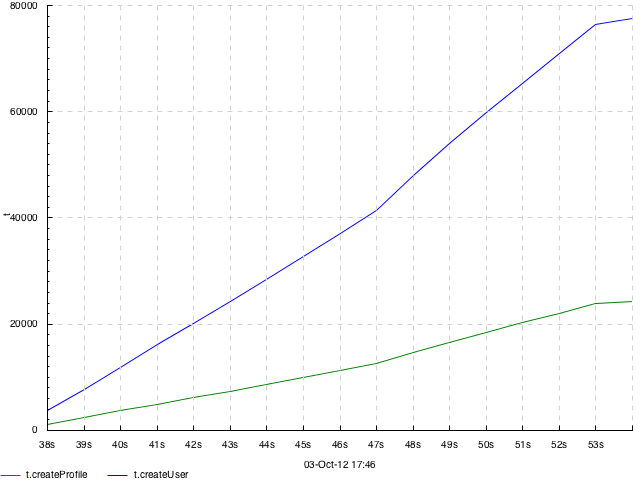
\includegraphics[width=0.5\textwidth]{pics/tplot/cumsum-create-user-and-profile-stacked.png}}

\pagebreak
\noindent
\textbf{Quantile plot~--- \texttt{quantile N $q_1,q_2,..,q_M$}}~--- slice time axis into N-second bins; draw a bar chart of $q_1$'th, $q_2$'th etc. percentiles of numeric values in each bin. All of $q_1$, $q_2$\ldots are numbers between 0 and 1. For example, 0.75 means the 75\% quantile, i.e. the value \emph{x} such that 75\% of the values in this bin are smaller than \emph{x}. Obviously, the 0'th quantile is the minimum value in the bin, and the 1'th quantile is the maximum value. 0 and 1 are always implicitly added to the quantiles you specify.

Specifically, within each bin, stacked bars of different color are drawn: $0..q_1$, $q_1..q_2$, \ldots, $q_M..1$. This means that the lower edge of what you see is the minimum value within that bin, and the upper edge is the maximum value; and bar boundaries correspond to the quantiles you asked for.

Example:

\centerline{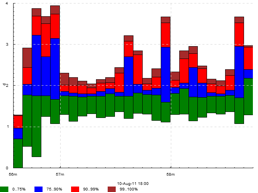
\includegraphics[width=0.5\textwidth]{pics/tplot/tplot-rmq-latency-2.png}}

This is a chart of kind \texttt{quantile 60 0.75,0.90,0.99}. The green bar spans from minimum in a bin to the 75\% quantile, the blue bar starts at 75\% and ends at 90\%, the red bar starts at 90\% and ends at 99\% and the brown bar starts at 99\% and ends at maximum. All this is reflected in the legend.

Another example:

\centerline{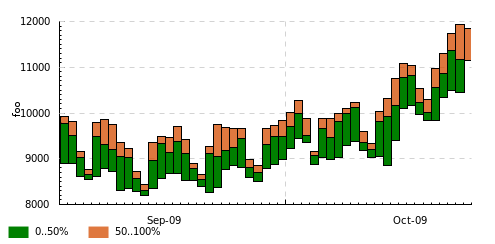
\includegraphics[width=0.5\textwidth]{pics/tplot/median.png}}

This was drawn with kind \texttt{quantile 86400 0.5}. The green bar spans from day minimum to median and the brown bar spans from median to day maximum.

\pagebreak
\noindent
\textbf{Bin frequency plot~--- \texttt{binf N $v_1,v_2,..,v_M$}}~--- slice time axis into N-second bins; draw a bar chart of frequencies of values falling into the bins $<v_1$, $v_1..v_2$, \ldots, $>v_M$. Frequencies are numbers from 0 to 1, so they add up to 1, so the total height of the bars is always 1.
\noindent
\textbf{Bin histogram plot~--- \texttt{binh N $v_1,v_2,..,v_M$}}~--- same as \texttt{binf}, but instead of frequencies, the absolute number of occurences of each bin is drawn.

Example of both \texttt{binf} and \texttt{binh}:

\centerline{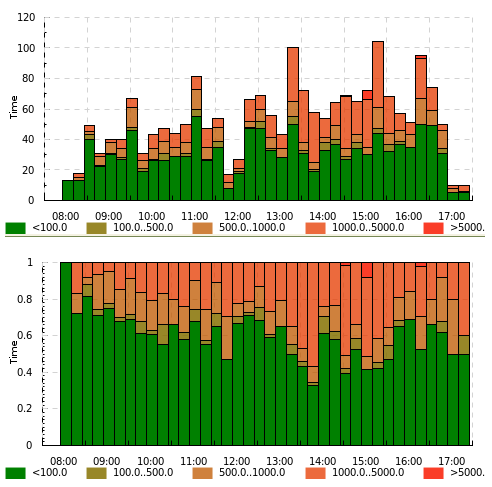
\includegraphics[width=0.8\textwidth]{pics/tplot/binf-binh.png}}

\emph{(this graph was made with an old version of \timeplot{} which had a pretty ugly color scheme\ldots)}

Here the same value (page download time by a web crawler) is drawn using both \texttt{binf} and \texttt{binh}: we see how frequently the download took below 100ms, 100 to 500ms, 500 to 1000ms etc. On the top graph we see \emph{what number} of pages took that much to download, and on the bottom graph we see \emph{what fraction} of pages took that much. In different situations both of these can be useful.

\pagebreak
\subsubsection{Kinds for counters}
\noindent
\textbf{Event plot~--- \texttt{event}}~--- draw intervals delimited by \texttt{>} and \texttt{<} input events and markers according to \texttt{@} and \texttt{!} events. In the more complex case where \texttt{>} and \texttt{<} do not strictly alternate, they are interpreted as ``+1'' and ``-1''-s to a counter and \timeplot{} draws intervals when the counter is greater than zero. Multiple input tracks per output track are not supported. If you need to draw something similar to what \texttt{event} does, but more complex, you might consider using \splot{} instead. \texttt{@TRACK COLOR} events act as \texttt{>} but the bar will have the indicated color. \texttt{!TRACK} will draw a vertical red dash and \texttt{!TRACK TEXT} will draw a red dash with a text label. 

Example:

\centerline{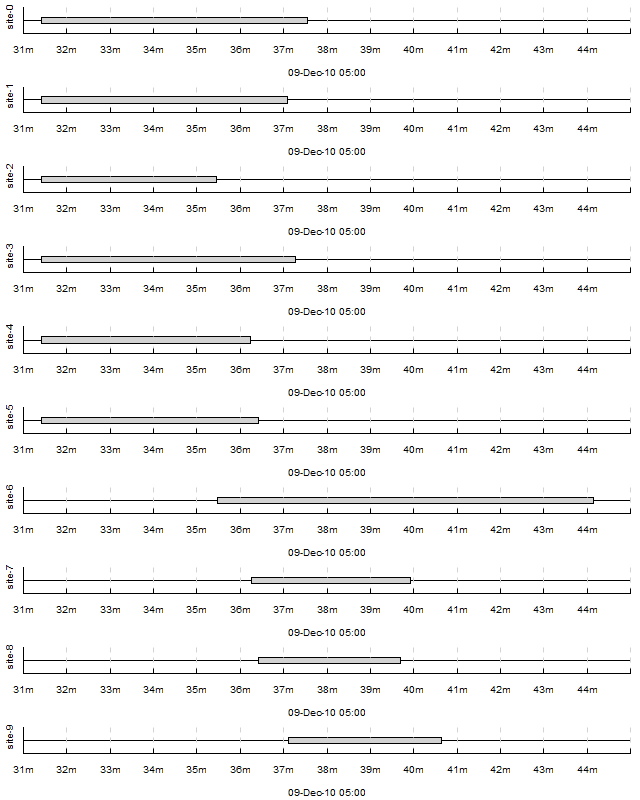
\includegraphics[width=0.8\textwidth]{pics/tplot/event.png}}

\pagebreak
\noindent
\textbf{Average count / activity count~--- \texttt{acount N}}~--- slice the time axis into N-second bins; draw histograms of the number of activities specified by \texttt{>}, \texttt{<} and \texttt{!} in each bin. More specifically:
\begin{itemize}
 \item Each input track mapping to this output track is interpreted as a counter
 \item \texttt{>} means ``+1'', \texttt{<} means ``-1'', \texttt{!} are counted separately
 \item In every bin, draw stacked bars: 1 bar per input track (with a consistent coloring across bins), height of the bar is average value of the counter + number of \texttt{!} events in this bin (usually you \emph{either} use \texttt{>} and \texttt{<}, \emph{or} \texttt{!}).
\end{itemize}

Example with 1 input track per output track: \texttt{acount 5}

\centerline{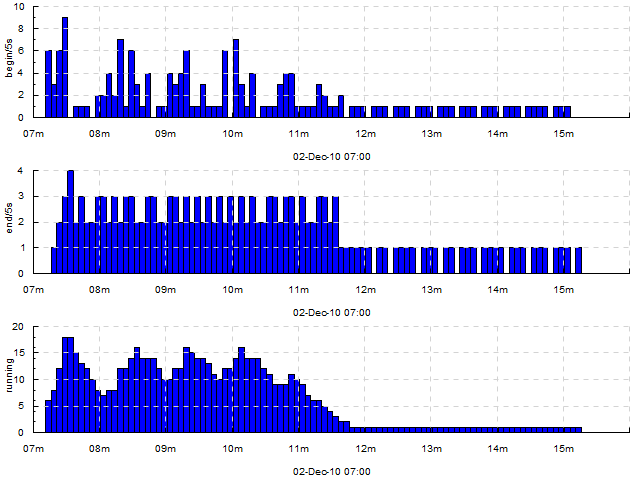
\includegraphics[width=0.8\textwidth]{pics/tplot/acount-begin-end-running.png}}

Here, we draw how many tasks are being 1) started 2) finished 3) being currently executed per every 5 seconds. The trace looked like this:

\begin{verbatim}
...
2010-12-02 07:08:15 !begin/5s
2010-12-02 07:08:15 >running
...
2010-12-02 07:08:18 !end/5s
2010-12-02 07:08:18 <running
...
\end{verbatim}

So, for the top two graphs we're counting \texttt{!} events and for the bottom graph we're looking at the average value of the counter bumped by \texttt{>} and \texttt{<}.

Example with two input tracks per output track: \texttt{within[.] acount 5}

\centerline{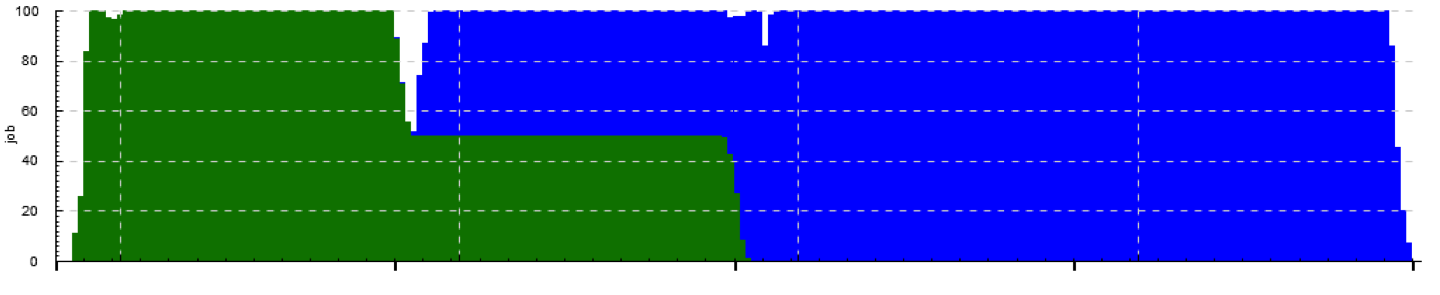
\includegraphics[width=0.8\textwidth]{pics/tplot/tplot-preemption.png}}

Here we see how the cluster is executing one job at full capacity, then another job comes in, preempts some of the first job's tasks and starts its own tasks there, etc. Each job's task starts are mapped to \texttt{>job.JOBID} and task completions are mapped to \texttt{<job.JOBID}.

Example with several input tracks per output track: \texttt{within[.] acount 5}

\centerline{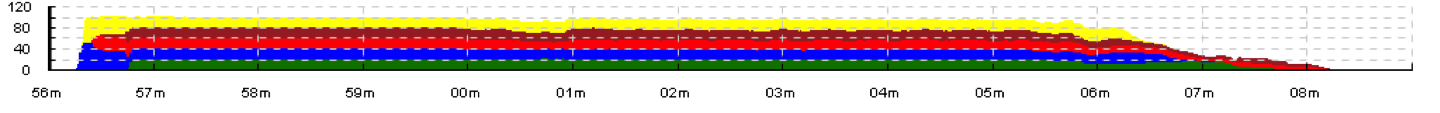
\includegraphics[width=0.8\textwidth]{pics/tplot/tplot-4rmq.png}}

Here, a single job is being executed on a cluster with a task queue sharded into 4 sub-queues. The graph shows the number of concurrently executing tasks taken from each shard over time (every worker is attached to a single shard; when a task starts on a worker attached to queue shard S, an event \texttt{>run.S} is emitted; when it finishes, \texttt{<run.S} is emitted). We see that some shards deplete later than others.

% Here, we have a lot of jobs executing on the cluster, the top graph shows how many sub-tasks of each job are in the task queue (sent by the producer but not yet received by the worker~--- sends are mapped to \texttt{>fly.JOBID} and receives are mapped to \texttt{<fly.JOBID}), and the bottom graph shows how many are concurrently executing (task starts are mapped to \texttt{>run.JOBID} and task completions are mapped to \texttt{<run.JOBID}).

\pagebreak
\noindent
\textbf{Average activity count as percentage~--- \texttt{apercent N X}}~--- exactly the same as \texttt{acount N}, but the Y axis is scaled into percentages of X. Useful if e.g. you have X cores and you're counting what percent of them are busy running tasks delimited by \texttt{>} and \texttt{<} at any given moment.

Example with both 1 and several input tracks per output track: \texttt{+k run 'apercent 60 420' +k run 'within[.] apercent 60 420'}

\centerline{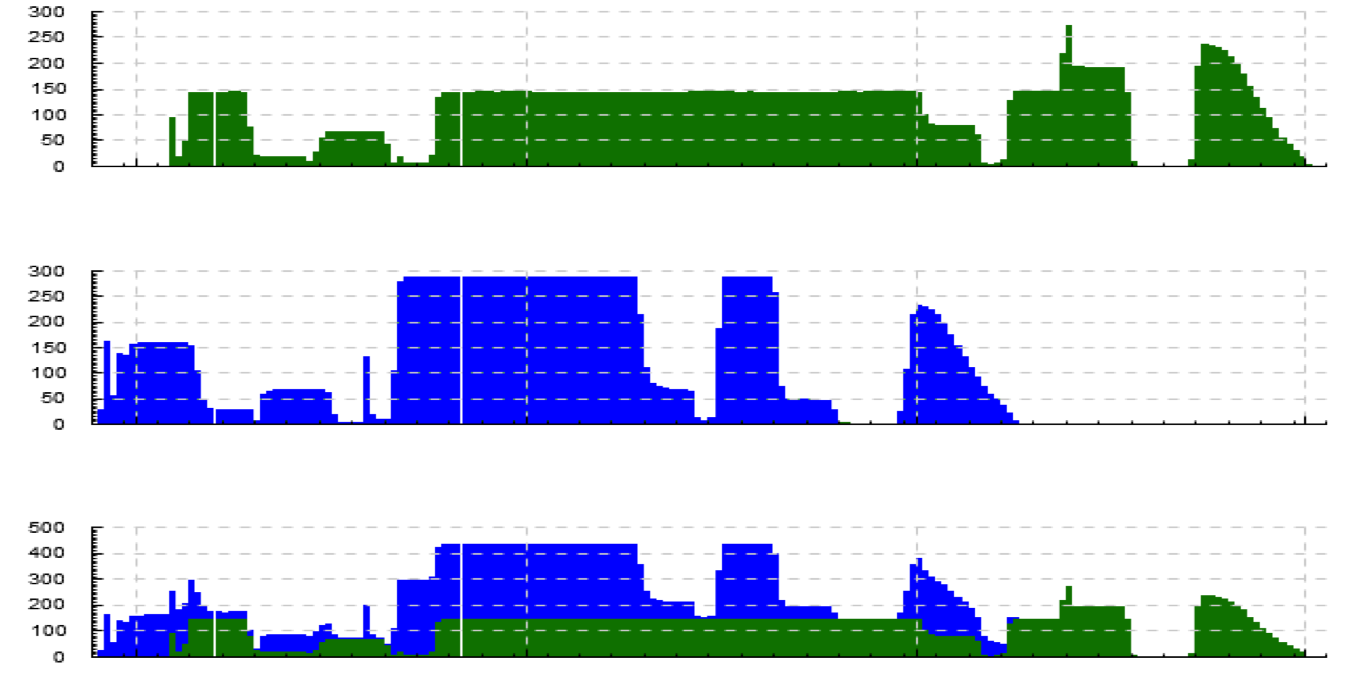
\includegraphics[width=0.8\textwidth]{pics/tplot/tplot-two-different-jobs-parallelization.png}}

\emph{The original log has been lost and only a picture with manually erased axis labels was left. Originally, there were labels on all axes. 1 tick on the X axis is actually 1 hour.}

Here, two jobs are being executed on a cluster with 420 cores. The graphs show utilization of the cluster (what percentage of cores are busy at any given moment) by both jobs separately and together. When a task starts, an event \texttt{>run.JOBID} is emitted; when a task completes, \texttt{<run.JOBID} is emitted. To understand how we get three plots here (1 per job and 2 for both together), see section \nameref{sec:tplot-track-mapping}.

\pagebreak
\noindent
\textbf{Average relative activity frequency~--- \texttt{afreq N}}~--- same as \texttt{acount N}, but in each bin the heights of bars for different input tracks are normalized to add up to 1. So, this graph is useless if you have just 1 input track mapped to the output track, but if you have many, it shows you the ratio between intensity of different activities.

Example with two input tracks per output track: \texttt{within[.] acount 5}

\centerline{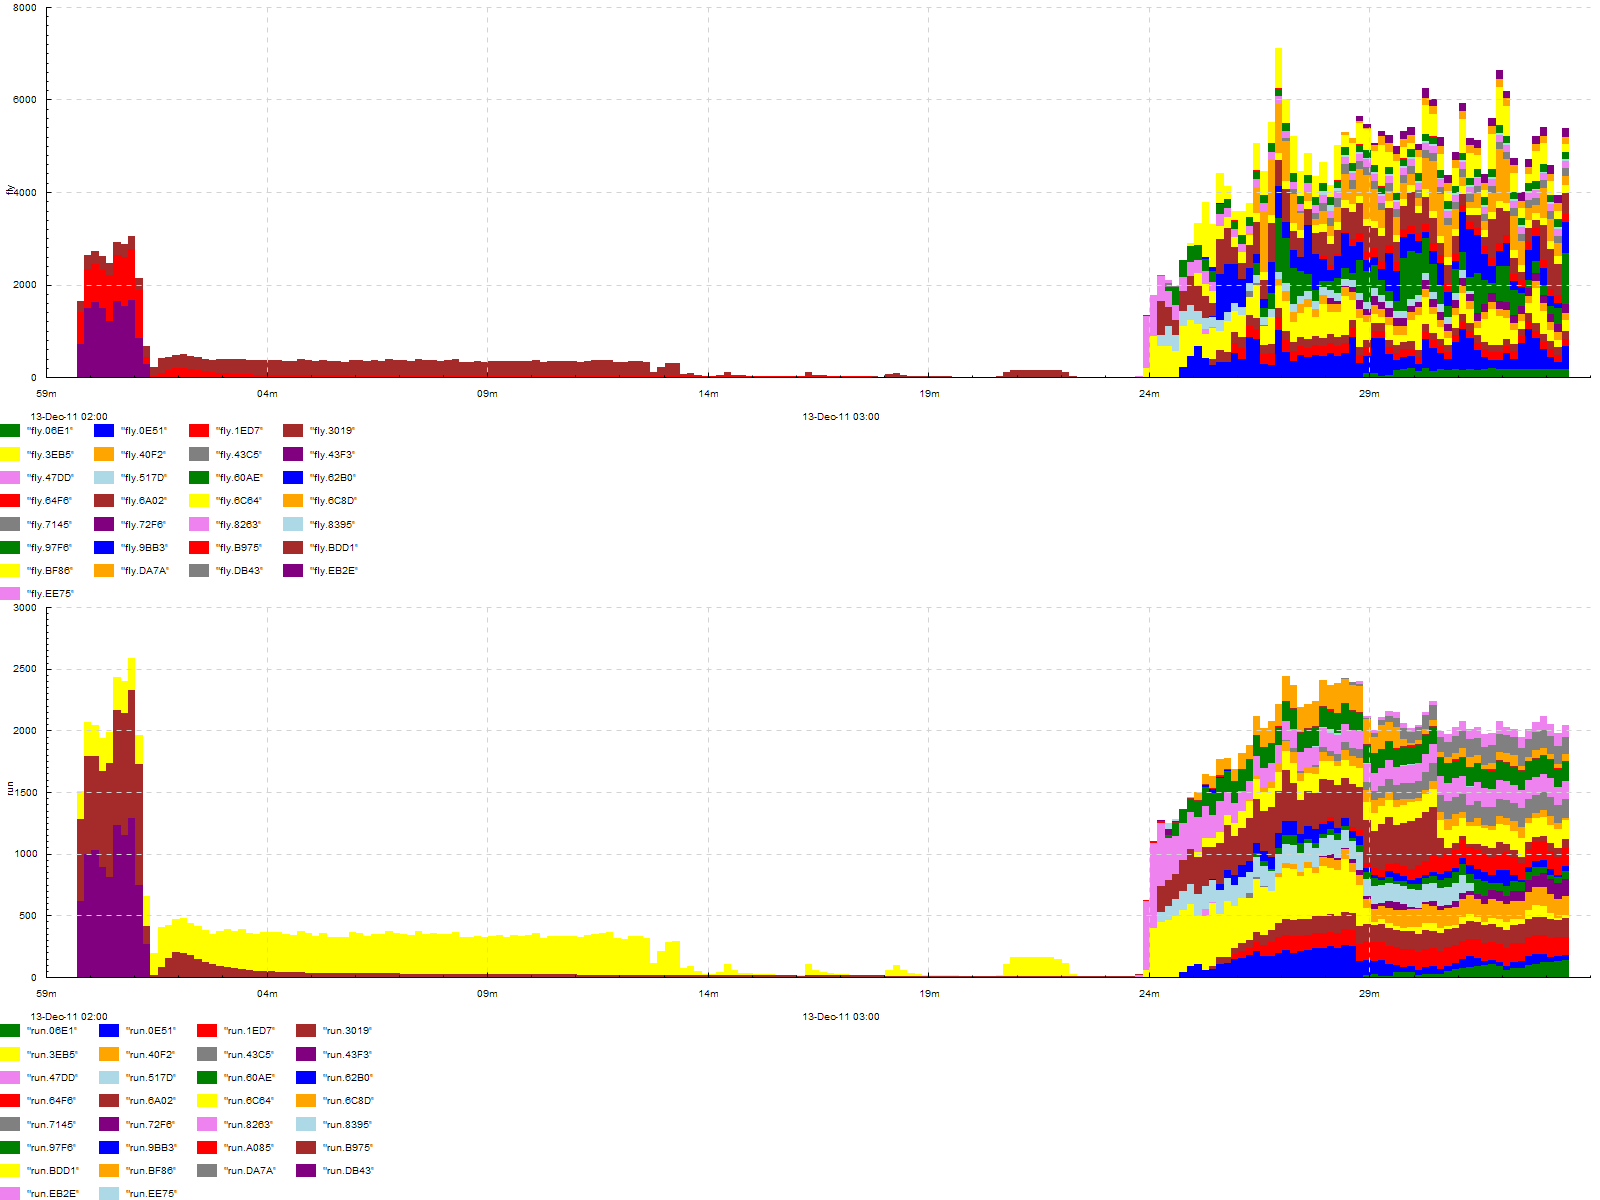
\includegraphics[width=0.8\textwidth]{pics/tplot/acount-fly-run-manyjobs.png}}

Here, two jobs are executing on the cluster, each job's task starts are mapped to \texttt{>absolute.JOBID} and \texttt{>relative.JOBID} and task completions are mapped to \texttt{<absolute.JOBID} and \texttt{<relative.JOBID}. Then \texttt{relative} is drawn with \texttt{within[.] afreq 5} and \texttt{absolute} with \texttt{within[.] acount 5}: \texttt{-k relative 'within[.] afreq 5' -k absolute 'within[.] acount 5'}\footnote{In the latest versions of \timeplot{} you don't need this data duplication, you can use \texttt{+k}~--- see section \nameref{sec:tplot-track-mapping}}. Both graphs illuminate different interesting aspects of the data.

\pagebreak
\subsubsection{Kinds for discrete data}
\noindent
\textbf{Discrete value frequency~--- \texttt{freq N TYPE}}~--- slice the time axis into N-second bind; within each bin, draw bars proportionally to the frequencies of different values of a discrete variable (\texttt{`} events). Multiple input tracks per output track are not supported. If TYPE is \texttt{clustered}, the bars are drawn next to each other; if TYPE is \texttt{stacked} (default), they are stacked vertically and add up to 1.
\noindent
\textbf{Discrete value histogram~--- \texttt{hist N TYPE}}~--- same as \texttt{freq N TYPE}, but absolute numbers of occuresnces of each value are drawn rather than the frequencies.

Example: \texttt{hist 60}

\centerline{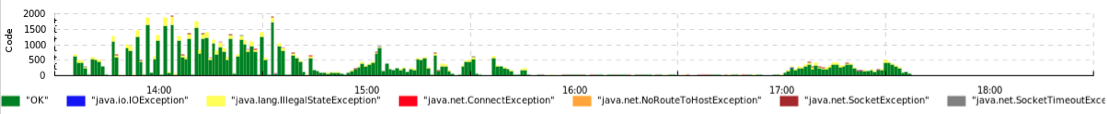
\includegraphics[width=0.8\textwidth]{pics/tplot/hist.png}}

Here, we draw the frequency of different outcomes of page downloads by a web crawler written in Java. The input trace consists of events like \texttt{=Code `OK}, \texttt{=Code `java.io.IOException} etc.

These two kinds can be emulated by \texttt{acount} and \texttt{afreq}: a chart of kind \texttt{freq N} over events \texttt{=foo `BAR} is equivalent to a chart of kind \texttt{within[.] afreq N} over events \texttt{!foo.BAR}.

\pagebreak
\subsection{Track and plot kind mapping}
\label{sec:tplot-track-mapping}
The process of mapping input events to output tracks consists of several steps. We'll understand it by describing the mapping algorithm and demonstrating it on a few simple examples involving the different parts of the algorithm.

Here's what happens to every input event (assume the event's input track is TRACK):
\begin{itemize}
\item Compare it to all the patterns among \verb|+k PATTERN '+SUF TYPE'|. For those that match:
\subitem If \verb|TYPE| is \verb|within[#] SUBTYPE|, and \verb|TRACK| is of the form \verb|BASE#SUB|, place the event onto output track \verb|BASE.SUF|.
\subitem Otherwise, place the event onto output track \verb|TRACK.SUF|.
\item Do the same for \verb|+dk '+SUF TYPE'|.
\item Do the same for the \emph{first} matching pattern among \verb|-k PATTERN '+SUF TYPE'|.
\item If no \verb|-k| patterns matched, do the same for \verb|-dk|.
\end{itemize}

To understand this, compare it to the simple special cases shown below.

\textbf{Simplest case, single input track and single plot type:} 1 input track, 1 plot kind mapping~--- the ``default'' mapping specified by \verb|-dk K|. This sole input track should be drawn with plot kind K (e.g. \verb|dots|). We'll have 1 dot plot in the output, showing events from the sole input track.

\textbf{Multiple input tracks, single plot type:} Several input tracks, 1 default plot kind mapping. We get several plots of the same type (e.g. several dot plots) vertically stacked with a common time axis. \textbf{For example:} if we have several memcached servers and we measure the durations of requests to them, we can have input tracks named \verb|rtime.mcd1|, \verb|rtime.mcd2| etc.

\textbf{Multiple input tracks with different plot types:} We wish to draw some input tracks with one plot type and some with another. We specify several regex/type mappings using \verb|-k PATTERN TYPE|. 

E.g. if we also have an input track \verb|cache| with discrete measurement events \verb|`HIT| and \verb|`MISS| and we wish to draw their rate, we can use \verb|-k rtime dots| \verb|-k cache 'freq 1'|. Then the output will have vertically stacked dot plots for tracks \verb|rtime.mcd1|, \verb|rtime.mcd2| etc, and a frequency plot for the track \verb|cache|. 

Input tracks that don't match any of the \verb|-k| patterns get drawn using the default plot type specified by \verb|-dk|.

\textbf{Single input track drawn with several different plot types:} We wish to make events from a single input track participate in multiple output plots, e.g. draw both the absolute and relative frequency of a track of discrete measurement events. Then we use \verb|+k PATTERN '+SUF TYPE'|. This means ``for tracks that match \verb|PATTERN|, append \verb|.SUF| to their name and draw a plot of type \verb|TYPE|''. 

For example: \verb|+k cache '+f freq 1'| \verb|+k cache '+h hist 1'| will produce two output tracks: \verb|cache.f| drawn with plot type \verb|freq 1| and \verb|cache.h| drawn with plot type \verb|hist 1|. Or, if (for some reason) you decide to draw both a dot and line plot of request times, you can try \verb|+k rtime '+dot dots'| \verb|+k rtime '+line lines'| and get tracks \verb|rtime.mcd1.dot|, \verb|rtime.mcd2.dot| \ldots drawn with \verb|dots| and \verb|rtime.mcd1.line|\ldots drawn with \verb|lines|. 

There's also \verb|+dk '+SUF TYPE'| with similar semantics. 

The suffixes are needed because otherwise the names of output tracks for the different plot types specified by \verb|+k| for a single input track would be identical, i.e. it would be the same output track, \timeplot{} cannot have two identically named output tracks. If the suffix is not specified (e.g. \verb|+k rtime dots|) it is assumed to be empty.

\textbf{Events from several similarly named input tracks drawn on a single plot:} Assume that you wish to draw dot plots of request times to different memcached servers not on several vertically stacked plots, but on a single dot plot, with different servers color-coded. Assume again that the input tracks are named \verb|rtime.SERVER|. 

Then you should use the \verb|within[SEP]| plot meta-type: \verb|-k rtime 'within[.] dots'|. This means: map input tracks to output tracks by dropping everything after the separator \verb|SEP|, in this case after \verb|.|, and we get a single output track \verb|rtime| to which go all the events from \verb|rtime.mcd1|, \verb|rtime.mcd2| etc. The plot type \verb|dots| will then take care of color-coding the different input tracks within a single output track. Other plot types deal with this situation in a sensible manner too, see section \nameref{sec:tplot-plot-kinds}.

\pagebreak
\subsection{Option reference}
\begin{longtable}{|l|p{160px}|l|}
\hline
\textbf{Option} & \textbf{Meaning} & \textbf{Default value} \\
\hline
\endhead
\verb|--help| & Show help & \\
\hline
\verb|--version| & Show version information & \\
\hline
\verb|-if INFILE| & Input filename. ``\texttt{-}'' means read from stdin. Do not use ``\texttt{-}'' for large inputs (above $\approx$100,000 events)! \timeplot{} can only work well on large inputs if it is in a file. & \emph{Required} \\
\hline
\verb|-o OUTFILE| & Output filename with extension & \emph{Required} \\
\hline
\verb|-of FORMAT| & Output format: \texttt{svg}, \texttt{png}, \texttt{pdf}, \texttt{ps} & Extension of \texttt{-o} \\
\hline
\verb|-or WIDTHxHEIGHT| & Output resolution, e.g. \texttt{640x480} & Extension of \texttt{-o} \\
\hline
\verb|-tf PATTERN| & Format of time in the input file as in \href{http://linux.die.net/man/3/strptime}{man strptime} but with fractional seconds supported via \verb|\%OS| - will parse \verb|12.4039| or \verb|12,4039|.  Also, \verb|%^[+-][N]s| will parse seconds since the epoch, for example \verb|%^-3s| are milliseconds since the epoch (N can only be 1 digit) & \verb|%Y-%m-%d %H:%M:%OS| \\
\hline
\verb|-dk KIND| & Default diagram kind. Do not forget to quote it! See section \nameref{sec:tplot-track-mapping}. & None \\
\hline
\verb|+dk KIND| & --- & None \\
\hline
\verb|-k PATTERN KIND| & Diagram kind for pattern PATTERN. See section \nameref{sec:tplot-track-mapping}. & None \\
\hline
\verb|+k PATTERN KIND| & --- & None \\
\hline
\verb|-fromTime TIME| & Filter events whose time is $\ge$ this time. Format specified by \texttt{-tf}. & None (no filter) \\
\hline
\verb|-toTime TIME| & Filter events whose time is $\le$ this time. Format specified by \texttt{-tf}. & None (no filter) \\
\hline
\verb|-baseTime TIME| & Draw time axis labels as seconds elapsed since TIME, instead of absolute time. Format specified by \texttt{-tf}. & \emph{Required} \\
\hline
\end{longtable}

\pagebreak
\subsection{Example data and exercises}
In this section we list some example datasources and exercises to try on them.

\subsubsection{Consumer power consumption.} \url{http://archive.ics.uci.edu/ml/datasets/Individual+household+electric+power+consumption}. This dataset contains measurements of power consumption of a single household, measuring several characteristics over the course of several years. It's in a simple CSV format which is described at the link. Beware: some data is not available and there are question marks in place of missing data items. You can completely skip such rows for the purpose of this exercise.

\textbf{Excerpt from the log:}
\begin{verbatim}
Date;Time;Global_active_power;Global_reactive_power;Voltage;Global_intensity;Sub_metering_1;Sub_metering_2;Sub_metering_3
16/12/2006;17:24:00;4.216;0.418;234.840;18.400;0.000;1.000;17.000
16/12/2006;17:25:00;5.360;0.436;233.630;23.000;0.000;1.000;16.000
16/12/2006;17:26:00;5.374;0.498;233.290;23.000;0.000;2.000;17.000
16/12/2006;17:27:00;5.388;0.502;233.740;23.000;0.000;1.000;17.000
16/12/2006;17:28:00;3.666;0.528;235.680;15.800;0.000;1.000;17.000
\end{verbatim}

\begin{tabular}{m{300px}V}
\hline
\emph{Exercise} & \emph{Expected result} \\
\hline
Make a dot plot of \verb|Voltage| for January 1st, 2007. Do not limit \emph{the trace}, use \verb|-fromTime| and \verb|-toTime|. & \thumbnail{pics/tplot/power-voltage.png} \\
Make a line plot of \verb|Global_active_power| vs \verb|Global_reactive_power| on one plot and a line plot of \verb|Voltage| on another (i.e., the result should be a stack of two plots), for January 1st, 2007. Use an opacity level of 0.5. & \thumbnail{pics/tplot/power-active-reactive-voltage.png} \\
Make a quantile plot, with quantiles of 0.1, 0.5 and 0.9 over bins of 1 day, for \verb|Global_active_power| and \verb|Global_reactive_power|, for the entire dataset. & \thumbnail{pics/tplot/power-active-reactive-quantile.png} \\
\hline
\end{tabular}

\subsubsection{Video encoding.} \emph{This dataset generously provided by Dmitry Popov.} \url{http://jkff.info/datasets/dmitry-popov-video-encoding.tar.gz}. This is a set of logs of a video encoding pipeline. For every video sample, the log contains times that this sample entered several steps of the pipeline: \verb|Grab1|, \verb|Grab2|, \verb|SR.YUV| and \verb|AviWr|. The three logs show how the same video was encoded with 3 versions of the program after different optimizations.

\textbf{Excerpt from the log:}
This excerpt shows all entries in the log \verb|1.txt| relating to sample \verb|[0]|. In the full log, entries for all samples are intermixed. Use column 1 as the timestamp.
\begin{verbatim}
0.000000 (0.000000) (0.000000) Grab1 sample [0] 0.000000, locking..
0.000006 (0.000006) (0.000006) Grab1 [0] got lock, carry on..
0.000611 (0.000604) (0.000611) Grab1 [0] sample processed.
0.000615 (0.000000) (0.000615) Par1.In received sample [0]
0.000629 (0.000000) (0.000629) SR.YUV got sample [0]
0.011636 (0.011007) (0.011636) SR.YUV done with sample [0]
0.011643 (0.000000) (0.011643) ParLast.In received sample [0]
0.011661 (0.000000) (0.011661) Grab2 sample [0] 0.000000, locking..
0.011666 (0.000005) (0.011666) Grab2 [0] got lock, carry on..
0.014947 (0.003280) (0.014947) Grab2 [0] sample processed.
0.598770 (0.000000) (0.598770) AviWr.V video sample [0] received
9.736371 (0.000466) (9.736371) AviWr.V [0] WriteVideo, locking..
9.736373 (0.000001) (9.736373) AviWr.V [0] got lock, writing..
9.736460 (0.000086) (9.736460) AviWr.V [0] write complete.
\end{verbatim}

\begin{tabular}{m{300px}V}
\emph{Exercise} & \emph{Expected result} \\
\hline
Plot the number of samples arriving per second to \verb|Grab1|, \verb|Grab2|, \verb|SR.YUV| and \verb|AviWr|. & \thumbnail{pics/tplot/thedeemon-acount.png} \\
Make an event plot, using impulse events for sample arrivals to these stages. Limit to the first 20 seconds. & \thumbnail{pics/tplot/thedeemon-event.png} \\
Make 4 dot plots for durations of processing at these stages. & \thumbnail{pics/tplot/thedeemon-dots.png} \\
Plot the same, but on a single plot (hint: use \verb|within|). & \thumbnail{pics/tplot/thedeemon-dots-all.png} \\
\end{tabular}

\subsubsection{DrWeb log}. \emph{This log was generously provided by Paul Graphov.} \url{http://jkff.info/datasets/paul-graphov-drweb.tar.gz}. This is a log of DrWeb Antivirus Server, and the most interesting entries in it are those relating to TCP data flow and to DB transactions:

% TODO Ask Paul if I understood the log format correctly.
\begin{verbatim}
20121024.114904.78 db3 [  415   448] mth:1  ...:ANTON-WIN7RU: data arrived, 32b
20121024.114904.78 tr2 [  415   448] mth:1  ...:ANTON-WIN7RU: rcv 17 GETTIME(6348666174470429760) 0b data
20121024.114904.78 db3 [  415   448] mth:1  ...:ANTON-WIN7RU: cancel timeout, GETTIME
20121024.114904.78 tr2 [  415   448] mth:1  ...:ANTON-WIN7RU: cmd (49b) "11 TIME 6348666174470429760 6348666174478278600"
20121024.114904.78 db3 [  415   448] mth:1  ...:ANTON-WIN7RU: cancel timeout, prolongate
20121024.114904.78 db3 [  415   448] mth:1  ...:ANTON-WIN7RU: set timeout to 60000 ms <6348666180478295800>
20121024.114904.78 db3 [  415   449] mth:2  ...:ANTON-WIN7RU: data arrived, 14b
\end{verbatim}

and

\begin{verbatim}
20121024.114904.78 db3 [  415   449] mth:2  [DB] Successful BEGIN transaction, 00.000 wait
20121024.114904.78 db3 [  415   449] mth:2  [IntDB] Statement "..."
20121024.114904.78 db3 [  415   449] mth:2  [DB] OK, 00.000, ...
20121024.114904.78 db3 [  415   449] mth:2  [IntDB] Statement "..."
20121024.114904.78 db2 [  415   449] mth:2  [DB] 1 row, 00.000, ...
20121024.114904.78 db3 [  415   449] mth:2  [IntDB] Statement "..."
20121024.114904.78 db2 [  415   449] mth:2  [DB] 79 rows, 00.000, ...
20121024.114904.78 db3 [  415   449] mth:2  [IntDB] Statement "COMMIT"
20121024.114904.78 db3 [  415   449] mth:2  [DB] Database has been freed but nobody wants it now 
20121024.114904.78 db3 [  415   449] mth:2  [DB] Successful COMMIT transaction, 3 statements, 00.000 wait, 00.000 execute, 00.000 commit 
\end{verbatim}

\begin{tabular}{m{300px}V}
\hline
\emph{Exercise} & \emph{Expected result} \\
\hline
Plot the data arrival rate (according to \verb|data arrived| entries) per 5-second bins (use \verb|sum|). & \thumbnail{pics/tplot/graphov-arrival.png} \\
Plot the transaction commit rate (according to \verb|Successful COMMIT| entries) per 5-second bins. & \thumbnail{pics/tplot/graphov-txcommit.png} \\
Plot the same transaction commit rate, but so that we can see how it adds up from contributions by different threads (\verb|mth:1|, \verb|pth:2| etc.). Limit to the interval from 12:00 to 13:00. & \thumbnail{pics/tplot/graphov-txcommit-bythread.png} \\
Same as above, \emph{and use the same trace file}, but make it 1 plot per thread type (\verb|mth|, \verb|pth|, \verb|dbv| etc., but still with a breakdown \emph{by thread} within each type's plot). & \thumbnail{pics/tplot/graphov-txcommit-bythreadtype.png} \\
\hline
\end{tabular}

\pagebreak
\subsection{Gallery}
\label{sec:tplot-gallery}
% TODO
% TODO Reference relevant sections

\pagebreak
\section{\splot{} ~--- visualizing behavior of many \mbox{concurrent processes}}

\splot{} draws a single Gantt-like chart with a birds-eye view of the activity of a number of concurrent processes, each of which may be in one of several different states at each moment (e.g. processing one of several jobs, or being in a particular stage of processing). 

The input to \splot{}, in the basic form, is a sequence of events ``activity started'', ``activity finished'' (specifying the timestamp and the process whose activity we're speaking about). Every event also includes a color with which to render the activity.

\subsection{Simple example}

This example has two tracks ``thread-1'' and ``thread-2'' and demonstrates most of the basic features.

\begin{verbatim}
2010-10-21 16:45:12.014 >thread-2 blue
2010-10-21 16:45:13.329 >thread-1 blue
2010-10-21 16:45:13.635 <thread-1
2010-10-21 16:45:13.800 <thread-2
2010-10-21 16:45:13.810 >thread-1 blue
2010-10-21 16:45:13.810 >thread-2 orange
2010-10-21 16:45:14.010 >thread-1 orange
2010-10-21 16:45:14.258 <thread-2
2010-10-21 16:45:14.623 <thread-1
2010-10-21 16:45:14.629 >thread-2 orange
2010-10-21 16:45:15.138 >thread-1 orange
2010-10-21 16:45:15.319 >thread-1 blue
2010-10-21 16:45:15.502 <thread-1 red
2010-10-21 16:45:15.502 !thread-1 black Hi there
2010-10-21 16:45:16.112 <thread-2
\end{verbatim}

Invoke \splot{}:
\begin{verbatim}
$ splot -if splot.simplest-example.trace \
        -o splot.simplest-example.png -w 400 -h 160
\end{verbatim}

Result:
\begin{figure}[h]
\center
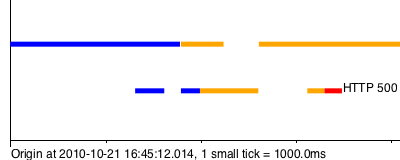
\includegraphics[scale=0.5]{pics/splot/splot-simplest-example.png}
\end{figure}

\pagebreak
\subsection{Motivation}
\label{sec:splot-motivation}
In this section we shall consider the plot we already saw in the introduction and see how it helps highlight a number of problems in the program whose behavior was visualized, that would be difficult to find without \splot{}.

{
\center
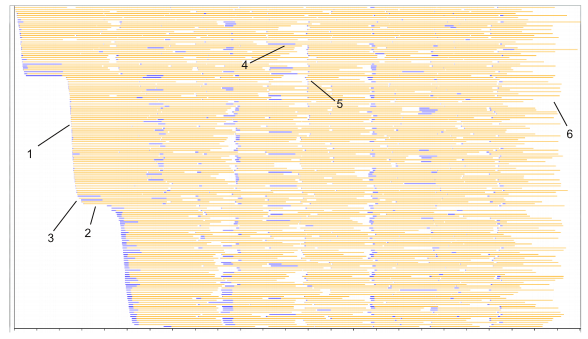
\includegraphics[width=\textwidth]{pics/splot/splot-main-example-analyzed.png}
}

Recall that here, the X axis is time, the Y axis is cluster worker (core), orange is computations and blue is fetching data from memcached.

There are several anomalies on this picture:

\vspace{3mm}

\textbf{1. Whitespace on the left: Slopes.} The beginning of the picture corresponds to the program startup~--- the first tasks are being fed into the shared queue and workers pick them up and start executing. The whitespace means that a large fraction of the program execution time is spent just warming up, while the workers essentially do nothing. The slopes mean that workers do not receive the first tasks instantly. Either it takes time to pick them from the queue, or they are being fed to the queue not quickly enough.

\textbf{2. Whitespace on the left: Plateaus.} The plateaus mean that there are moments when no tasks are being picked up at all. Either the queue is hung up, or the task producer. We also see how big an impact this has on the overall cluster utilization: a single 1-second plateau is worth 160 seconds of computations (as there are 160 workers on this picture)!

\textbf{3. The slope on the left is nonlinear.} The slope becomes less vertical at the end of each slope line. This means that task pickup rate (or perhaps task generation rate) is not constant. There's a ``tail'' in task delivery times. 

\textbf{4. Some blue bars are rather long.} This means that memcached fetches sometimes take a long time~--- comparable with computation time. We should optimize them.

\textbf{5. Vertical patterns of white space and blue bars lining up on their left edge.} This means that there are moments when everyone's got nothing to do and the task queue is empty, and then suddenly a lot of tasks appear in the queue and everyone is busy again. This is probably a problem with the task producer~--- maybe it is sending tasks in batches, or something like that.

\textbf{6. A lot of white space on the right.} This means that in the end of the program execution, when all tasks are already in the queue and no new ones will appear, a lot of time is spend when faster workers wait for slower workers. The program finishes when the very last worker finishes. The fraction of this whitespace is very well worth 5-10\% of the total program time. This anomaly is called ``the long tail effect'' and can be eased by increasing the task granularity (i.e. submitting many short tasks rather than several long ones). However, this will obviously increase load on the queue, so we have a trade-off here.

\vspace{3mm}

We see that a simple picture of the cluster behavior showed us quite a few non-trivial things, most of which would be very difficult to find without a visualization.

\pagebreak
\subsection{Concepts}

Let us now consider in detail all the concepts necessary to understand and use \splot{}.

\begin{description}
\item[Track (also process)] An entity which changes its state between several values (performs several activities) over time. At any moment, a process is doing at most one activity. We're usually interested in seeing the visual pattern emerging between different tracks. For example, it is often meaningful to assign 1 track = 1 thread in a multi-threaded program (in a distributed program one should of course include the machine into the track id).
\item[Activity] A period during which a process is in a particular problem-specific logical state. A single activity is drawn with a single color, as a bar which is horizontally as long as the activity (if there are a lot of tracks, this bar can be as thin as a hairline). For example, if we have a program whose threads are either computing, doing IO or waiting idly, we may depict the `computing' activity with orange color, IO as blue and idle waiting as lack of activity (no color at all).
\item[Event] Mark of the beginning or end of an activity on a particular track, specifying the activity's color. There are also ``text'' events which allow to draw text markers above the usual colored bars. An event has a timestamp, track and event type (activity start / activity end / text). For example, when our hypothetical program starts doing IO in thread T, we should represent this in \splot{}'s input as an event ``start blue activity on track ''.
\item[Color] Colors in \splot{} can be specified in several ways. In the simplest form, it can be an SVG color name or hex code (e.g. ``red'' or ``lightblue'' or ``\#ff0033''), it can be an arbitrary string (then a random color will be generated so that different strings correspond to different colors~--- this is useful to color-code an unknown number of different types of activities, e.g. if you have worker processes servicing several clients and you wish to get a picture of who services whom and color-code the clients: ``client-5''), and it can be an arbitrary string within a color scheme (e.g. ``/success/client-5'' or ``/failure/client-5'', and you might define the ``success'' colorscheme to consist of several greenish colors and ``failure'' of reddish).
\item[Color scheme] A list of colors which will be cycled between when generating colors for tracks whose color is not specified explicitly by a SVG color name or hex code.
\end{description}

\pagebreak
\subsection{Input format}

The input to \splot{} consists of a series of events.
\vskip3px
\begin{tabular}{|l|p{200px}|}
\hline
Format & Meaning \\
\hline
\verb|TIME >TRK COLOR| & Start activity of color COLOR on track TRK at time TIME (if there already is an activity, finish it and start a new one instead). \\
\hline
\multicolumn{2}{|l|}{\texttt{2010-10-21 16:45:09,431 >r2b3.t5 blue}} \\
\hline
\verb|TIME <TRK| & Finish the current activity of track TRK at time TIME \\
\hline
\multicolumn{2}{|l|}{\texttt{2010-10-21 16:45:10,322 <r23.t5}} \\
\hline
\verb|TIME <TRK COLOR| & Finish the current activity of track TRK at time TIME, overriding the color it was given at the start by COLOR. This is useful, e.g. do indicate that an activity failed by drawing it with red color (obviously when the activity begins, we don't know if it will fail or not). \\
\hline
\multicolumn{2}{|l|}{\texttt{2010-10-21 16:45:10,322 <r2b3.t5 red}} \\
\hline
\verb|TIME !TRK COLOR TXT| & Draw text TXT with color COL on track TRK, left-justified at time TIME \\
\hline
\multicolumn{2}{|l|}{\texttt{2010-10-21 16:45:10,322 !r2b3.t5 black read()}} \\
\hline
\end{tabular}

\pagebreak
\subsection{Advanced features}

\subsubsection{Bar height}
Bar height is specified with \verb|-bh|: either \verb|-bh fill| or \verb|-bh HEIGHT| (e.g. -bh 5). \verb|fill| means ``set bar height to fill the whole vertical space''. Consider the previous simple example, here it is with \verb|-bh fill|:

\begin{figure}[h]
\center
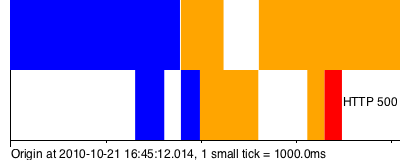
\includegraphics[scale=0.5]{pics/splot/splot-simplest-example-fill.png}
\caption{A trivial example of \splot{} usage with the \texttt{-bh fill} option}
\end{figure}

\verb|-bh fill| is vital when you have a lot of tracks (at least dozens). Perhaps it should be the default.

\subsubsection{Expiring activities~--- if \texttt{<} is missing}

In systems where components can crash (which is, most systems :) ), it might happen so that your log catches only the beginning of an activity but not its end, because the component has crashed in the middle. You can tell \splot{} ``expire all activities if they take longer than X seconds'' by using \verb|-expire X|; then, if an activity has not finished within X seconds, \splot{} will draw a dashed line and an X marker, meaning that the process probably crashed somewhere on the dashed line\footnote{It's probably meaningful to specify expiration times for each activity separately, but currently \splot{} has just a single global option}.

Consider a small example similar to the one we had before.

\begin{verbatim}
2010-10-21 16:45:12.014 >worker-2 blue
2010-10-21 16:45:13.329 >worker-1 blue
2010-10-21 16:45:13.635 <worker-1
2010-10-21 16:45:13.800 <worker-2
2010-10-21 16:45:13.810 >worker-1 blue
2010-10-21 16:45:13.810 >worker-2 orange
2010-10-21 16:45:14.010 >worker-1 orange
2010-10-21 16:45:14.258 <worker-2
2010-10-21 16:45:14.623 <worker-1
2010-10-21 16:45:14.629 >worker-2 orange
2010-10-21 16:45:15.138 >worker-1 orange
2010-10-21 16:45:15.319 >worker-1 blue
2010-10-21 16:45:16.512 <worker-2
2010-10-21 16:45:18.412 >worker-2 blue
2010-10-21 16:45:20.112 <worker-2
\end{verbatim}

Let us draw it with an expiration time of 2000 milliseconds:

\begin{verbatim}
$ splot -if splot.expire-example.trace -o splot-expire-example.png \
        -expire 2000 -bh 15 -w 400 -h 160
\end{verbatim}

Here's what we get:

\begin{figure}[h!]
\center
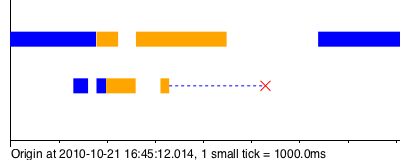
\includegraphics[scale=0.5]{pics/splot/splot-expire-example.png}
\caption{Using the \texttt{-expire} option with \splot{}}
\end{figure}

Here we see that perhaps ``worker-1'' (here drawn second, as its first event happened later than worker-2's) crashed and that's why it didn't do anything in the later parts of the graph.

Figure \ref{fig:splot-expire-large-example} shows a more complex real-life example from a cluster (the input log has unfortunately been lost). Here a large number of workers are preempted at once.

\begin{figure}
\center
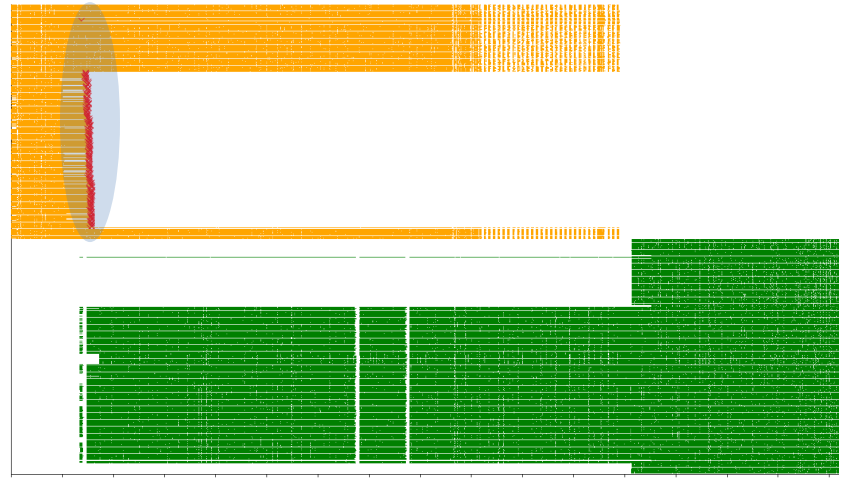
\includegraphics[width=\textwidth]{pics/splot/splot-expire-large-example.png}
\caption{Using the \texttt{-expire} option with \splot{}: a real-life example}
\label{fig:splot-expire-large-example}
\end{figure}

\subsubsection{Phantom color~--- if \texttt{>} is missing}

Sometimes you process logs which start in the middle of the program's execution, so the log doesn't catch the beginning events of activities that were active at the moment the log was started (however, the log \emph{does} catch their finishing events). \splot{} can display such ``phantom'' activities in a color of your choice, using the \verb|-phantom COLOR| option. Specifically, if a track starts with a \texttt{<} event instead of \texttt{>}, then \splot{} will assume that there was a \texttt{>} event with color COLOR in the past on this track.

Consider the same example as above, but let us cut it in the beginning, as if we had a truncated log:

\begin{verbatim}
2010-10-21 16:45:14.010 >worker-1 orange
2010-10-21 16:45:14.258 <worker-2
2010-10-21 16:45:14.623 <worker-1
2010-10-21 16:45:14.629 >worker-2 orange
2010-10-21 16:45:15.138 >worker-1 orange
2010-10-21 16:45:15.319 >worker-1 blue
2010-10-21 16:45:16.512 <worker-2
2010-10-21 16:45:18.412 >worker-2 blue
2010-10-21 16:45:20.112 <worker-2
\end{verbatim}

Now invoke \splot{}:
\begin{verbatim}
$ splot -if splot-phantom-simple-example.trace \
        -o splot-phantom-simple-example.png \
        -phantom gray -w 400 -h 160 -bh 5 
\end{verbatim}

And here's what we get:

\begin{figure}[h!]
\center
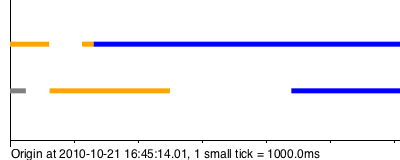
\includegraphics[scale=0.5]{pics/splot/splot-phantom-simple-example.png}
\caption{Using the \texttt{-phantom} option with \splot{}}
\end{figure}

We see a gray bar in the beginning of worker-2's track. This is because the first event on this track was \verb|2010-10-21 16:45:14.258 <worker-2|, i.e. an activity closing event, which means that the opening event was missed.

\subsubsection{Color auto-generation}

How do we color-code activities in \splot{}'s input if the set of possible activity types is not known in advance? E.g. you have a set a of worker processes which service a fairly small but unknown number of clients. You assign tracks to worker processes, and you wish to color-code the clients to see a picture of who services whom and when.
\\
In this case, you can simply use the client's id as color: for colors that do not parse as SVG color names or hex codes, \splot{} will generate a random color from a default contrast color scheme.
\\
Let us consider a real-life example. In this example, again some workers are processing tasks, but from different clients.
The trace looks like this:
\begin{verbatim}
...
2011-07-27 02:42:03.485 <RACK5UNIT067.37dc
2011-07-27 02:42:03.492 >RACK2UNIT067.4ca8 8610
2011-07-27 02:42:03.495 >RACK4UNIT075.5b15 8610
2011-07-27 02:42:03.496 >RACK4UNIT067.ec72 877B
2011-07-27 02:42:03.496 >RACK4UNIT067.f3fe 877B
2011-07-27 02:42:03.496 >RACK5UNIT017.0c21 8610
2011-07-27 02:42:03.498 >RACK2UNIT030.9e7a 071C
...
\end{verbatim}
So, we use track names of the form \verb|MACHINE.WORKERID| and instead of using color at \texttt{>} events, we use the client ID, asking \splot{} to color-code clients for us. The result is shown on figure \ref{fig:splot-color-gen}. Here red color denotes tasks that completed unsuccessfully and other colors (e.g. green and blue; red is excluded from the default color scheme precisely for situations like this) encode different clients\footnote{Yes, as this rather crazy picture might hint, the program \emph{did} have lots of problems~--- exposing them, that's what \splot{} is for.}.

\begin{figure}[h]
\center
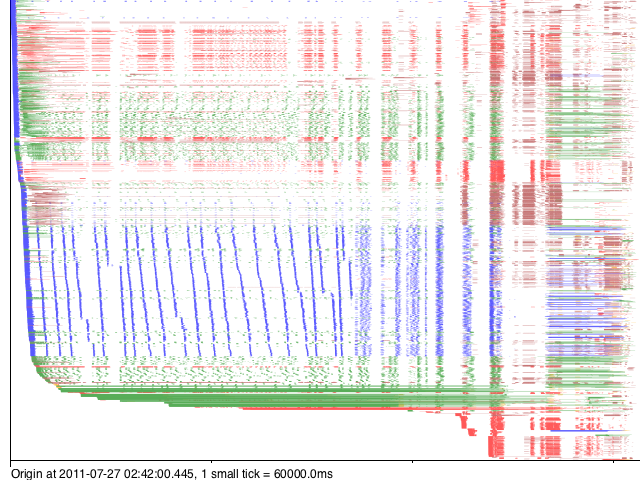
\includegraphics[width=\textwidth]{pics/splot/splot-color-gen.png}
\caption{Automatic color generation with \splot{}}
\label{fig:splot-color-gen}
\end{figure}

Assume the same case as above with worker processes servicing different clients. Assume also that worker processes might be in two modes: regular and workstealing (if they have nothing to do with their current client, they try to service tasks of some other client). We wish to depict regular tasks and tasks picked by work-stealing in different shades: e.g. regular tasks as bright colors and work-stolen ones as pale. We still wish to use color generation for both. This can be achieved by using color schemes. Specifically, we'll color-core regular tasks by \verb|TIMESTAMP >WORKER CLIENT| and work-stolen tasks by \verb|TIMESTAMP <WORKER /ws/CLIENT|. This tells \splot{} to generate colors for regular tasks from the default color scheme and for work-stolen tasks from the \verb|ws| color scheme, which we must specify in \verb|-colorscheme| parameters, e.g. \verb|-colorscheme ws='lightblue lightgray lightgreen pink beige'| (use more colors if you wish to distinguish between more clients).

\emph{(unfortunately, an example log illustrating this has been lost)}

\subsection{Option reference}

\begin{longtable}{|l|p{160px}|l|}
\hline
Option & Meaning & Default value \\
\hline
\endhead
\verb|-if INFILE| & Input filename & \emph{Required} \\
\hline
\verb|-o PNGFILE| & Output filename & \emph{Required} \\
\hline
\verb|-w WIDTH|   & Output width, pixels & \verb|640| \\
\hline
\verb|-h HEIGHT|  & Output height, pixels & \verb|480| \\
\hline
\verb|-bh BARHEIGHT| & Vertical height of each track's activity bars, pixels, or \verb|fill| to use all the available vertical space & \verb|fill| \\
\hline
\verb|-tf PATTERN| & Format of time in the input file as in \href{http://linux.die.net/man/3/strptime}{man strptime} but with fractional seconds supported via \verb|\%OS| - will parse \verb|12.4039| or \verb|12,4039|.  Also, \verb|%^[+-][N]s| will parse seconds since the epoch, for example \verb|%^-3s| are milliseconds since the epoch (N can only be 1 digit) & \verb|%Y-%m-%d %H:%M:%OS| \\
\hline
\verb|-tickInterval MILLIS| & Ticks on the X axis will be this often & \verb|1000| \\
\hline
\verb|-largeTickFreq N| & Every N'th tick will be larger than the others & \verb|10| \\
\hline
\verb|-sort SORT| & Sort tracks by time of first event (\verb|-sort time|) or by track name (\verb|-sort name|)~--- see ``track sorting'' above & \verb|name| \\
\hline
\verb|-expire MILLIS| & Expire activities that do not finish within MILLIS milliseconds~--- see ``expiring activities'' above & \emph{none (don't expire)} \\
\hline
\verb|-phantom COLOR| & Set the phantom color which is used if the first event on a track is \texttt{<}~--- see ``phantom color'' above & \emph{none (no phantom color)} \\
\hline
\verb|-fromTime TIME| & Clip the picture on the left (time in the format of \verb|-tf|, i.e. same as in the input) & \emph{none (don't clip)} \\
\hline
\verb|-toTime TIME| & Clip the picture on the right (time in the format of \verb|-tf|, i.e. same as in the input) & \emph{none (don't clip)} \\
\hline
\verb|-numTracks N| & Explicitly specify the number of tracks for better performance on very large data (see section ``Performance'' below) & \emph{none (compute from input)} \\
\hline
\verb|-colorscheme SCHEME COLORS| & Declare a colorscheme (see ``Color schemes'' above). Can be used multiple times. Scheme is an arbitrary string, e.g. \verb|pale| or \verb|bright|. COLORS is a space-separated list of colors in SVG or hex, e.g. \verb|'red green 0x0000FF'| & \emph{none} \\
\hline
\end{longtable}

\subsection{Gallery}
Figures \ref{fig:splot-gallery-first}--\ref{fig:splot-gallery-last} show a number of pictures produced by \splot{} in various real-life situations. Most of them look really creepy and expose different kinds of performance problems in the programs whose behavior they depict. The author already does not remember the precise reasons for the problems~--- think of it as a horror museum exposition and use your imagination.

\begin{figure}[p]
\center
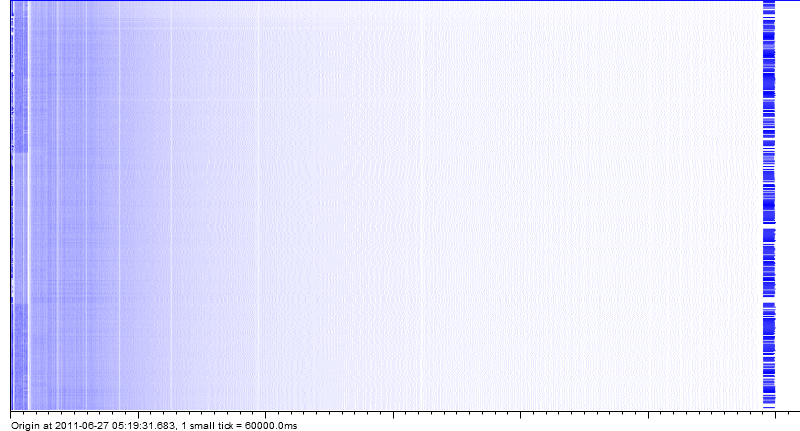
\includegraphics[width=0.8\textwidth]{pics/splot/gradient.png}
\caption{Blue: working, white: waiting. The task queue's performance was gradually becoming worse and worse.}
\label{fig:splot-gallery-first}
\end{figure}

\begin{figure}[p]
\center
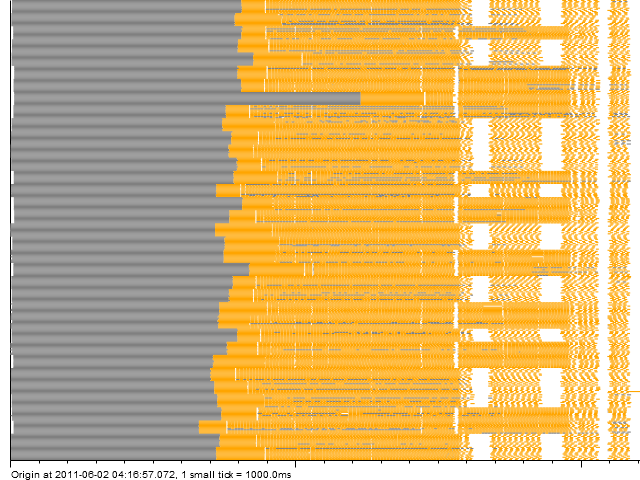
\includegraphics[width=0.8\textwidth]{pics/splot/creepy-startup.png}
\caption{Orange: working, gray: starting, white: waiting. The first time a program loads, it takes a long time. Loads on the same machine take the same time~--- .NET DLL caching (here the sort-by-track-name option is used, currently absent until reimplemented).}
\end{figure}

\begin{figure}[p]
\center
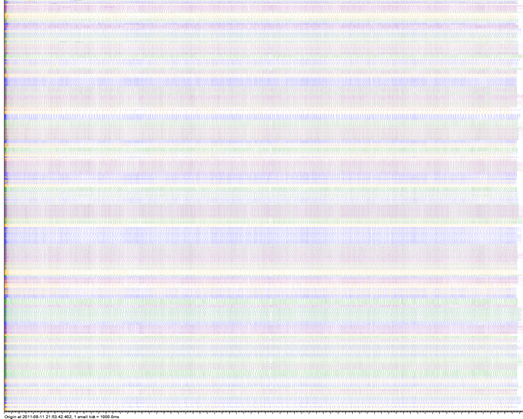
\includegraphics[width=0.8\textwidth]{pics/splot/4-rabbits.png}
\caption{Colors encode which shard of a task queue was being used. Initially the shards are fast, then they run slower but smoothly. Everything's fine.}
\end{figure}

\begin{figure}[p]
\center
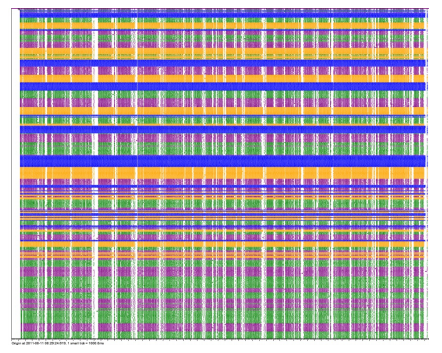
\includegraphics[width=0.8\textwidth]{pics/splot/rabbit-collision.png}
\caption{Colors encode which shard of a task queue was being used. Green and purple have problems, yellow and orange don't. Turned out green and purple corresponded to the same physical queue server which had to sustain double load.}
\end{figure}

\begin{figure}[p]
\center
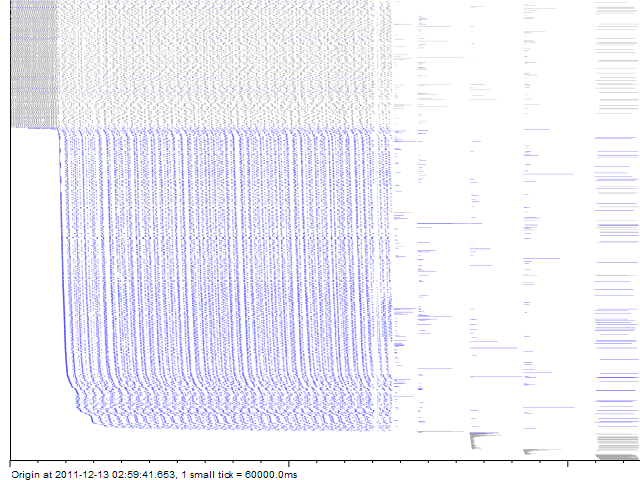
\includegraphics[width=0.8\textwidth]{pics/splot/workstealing.png}
\caption{Gray: normal tasks, blue: tasks picked by workstealing. After some period, workstealing begins and many workers start processing the job~--- slowing down the queue, but total throughput is higher.}
\end{figure}

\begin{figure}[p]
\center
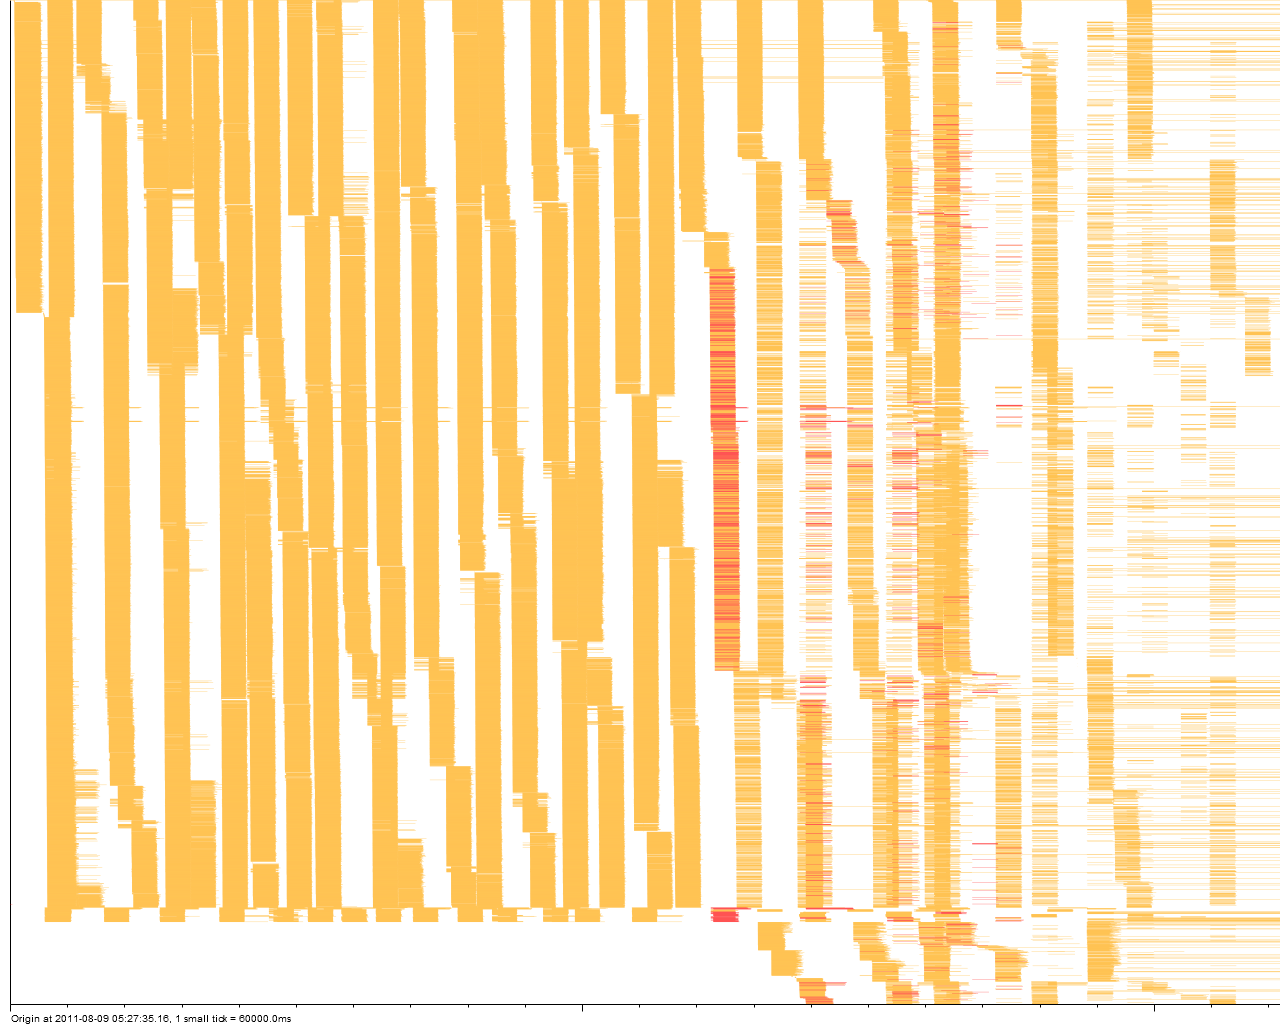
\includegraphics[width=0.8\textwidth]{pics/splot/creepy-prefetch.png}
\caption{Orange: working, red: preempted and lost work. The task queue prefetch feature was broken, leading to very strange patterns of task queue utilization.}
\end{figure}

\begin{figure}[p]
\center
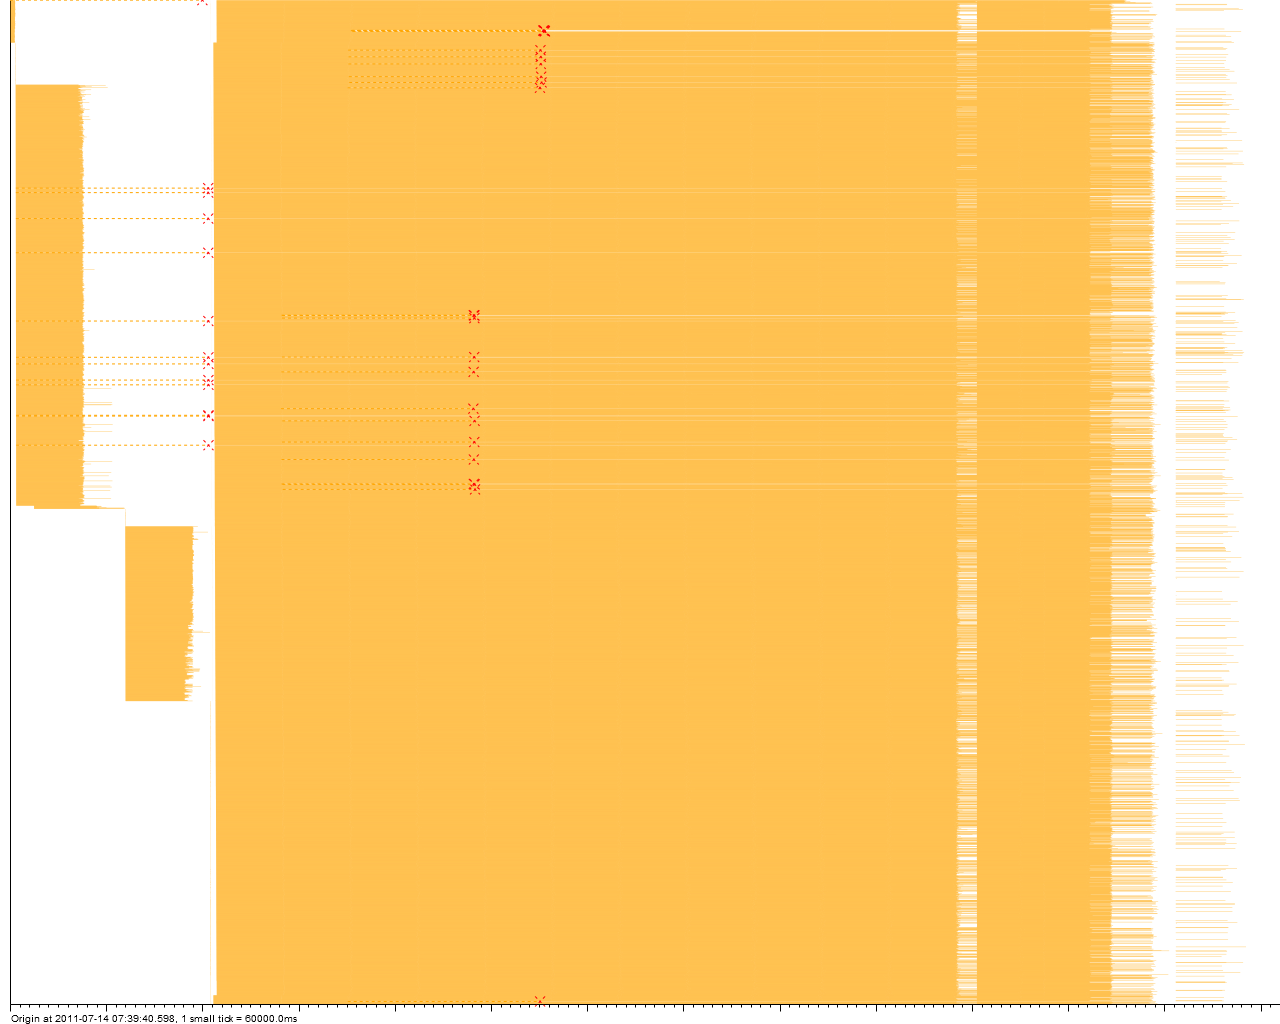
\includegraphics[width=0.8\textwidth]{pics/splot/simple-2stage-job.png}
\caption{A simple 2-stage job: a couple of insufficiently parallel data preparation steps, then a long stream of tasks utilizing the cluster well. Two worker machines died in the process.}
\end{figure}

\begin{figure}[p]
\center
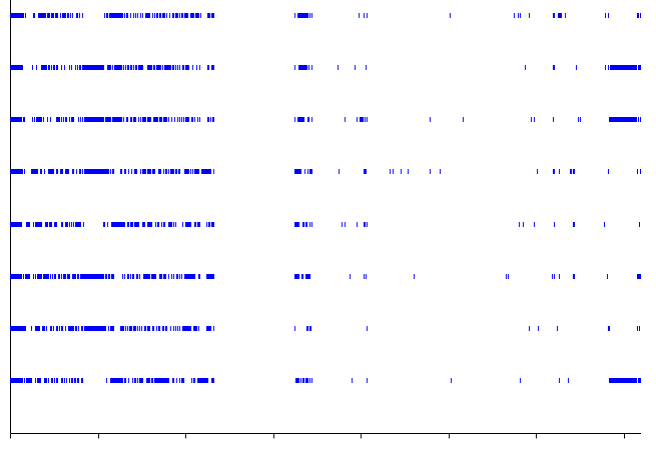
\includegraphics[width=0.8\textwidth]{pics/splot/8threads.png}
\caption{Bars correspond to a web service being called from different threads. Apparently there are periods when it takes longer, and periods when it's not called at all.}
\end{figure}

\begin{figure}[p]
\center
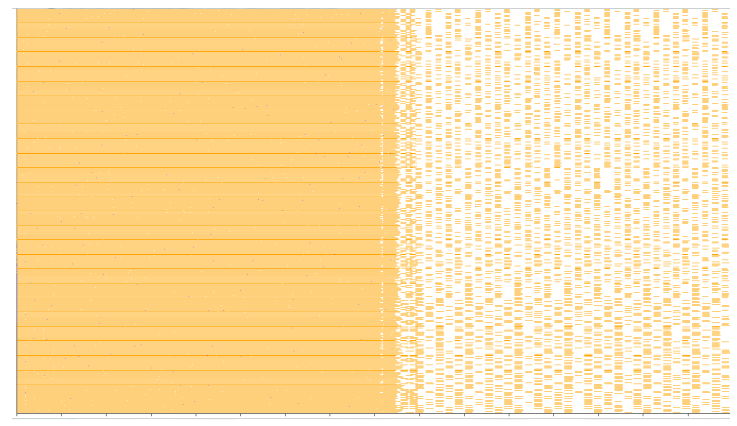
\includegraphics[width=0.8\textwidth]{pics/splot/njobs-then-one.png}
\caption{Several jobs run concurrently and saturate the cluster. Then all but one finish, and the one remaining runs in bursts of tasks, these bursts being not parallel enough to saturate the cluster (I recall it was a 480-core cluster and 160-task bursts).}
\end{figure}

\begin{figure}[p]
\center
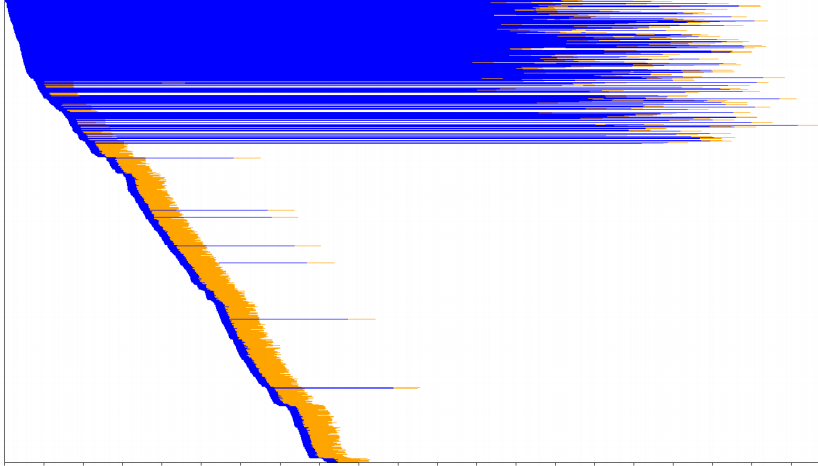
\includegraphics[width=0.8\textwidth]{pics/splot/very-slow-memcached.png}
\caption{Orange: working, blue: fetching from memcached. We see that early calls to memcached take a ridiculous amount of time. Later calls sometimes take long too, but not that long (I recall the reason was a broken retry mechanism).}
\end{figure}

\clearpage

\begin{figure}[p]
\center
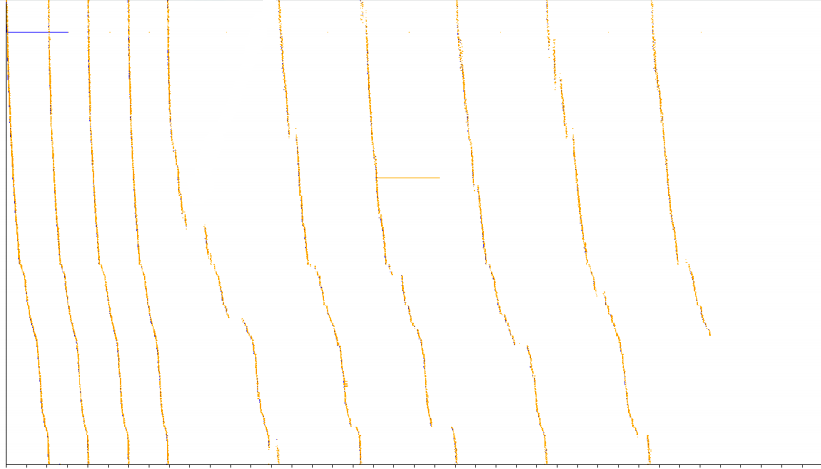
\includegraphics[width=0.8\textwidth]{pics/splot/spray.png}
\caption{There are 1900 tracks (cluster cores) here. The tasks that we put into the shared queue are by far too short, so the queue (and perhaps the task producer) becomes the bottleneck. We also see that the queue feeds tasks to workers in round-robin. And we also see that it slows down over time. And small pauses in the queue or task producer cost an awful amount of computing time because everyone is waiting for them.}
\label{fig:splot-gallery-last}
\end{figure}

\pagebreak

\section{Acknowledgements}

The following people contributed code to the tools or provided help otherwise at different times.
\begin{itemize}
\item Tim Docker wrote the excellent \textbf{Chart} library, on which \timeplot{} is based.
\item Ivan Tarasov promoted the tools, hosted an event where I could talk about them, and made a fork with a quantile graph with a log scale.
\item Arnaud Bailly found a large number of important bugs.
\item Dmitry Astapov and Julia Astakhova gave a lot of feedback.
\item Orion Jankowski did a pullrequest which exposed a number of bugs.
\item Jason Dusek, Ilya Teterin, Julia Chertkova gave examples of their usage of \timeplot{}.
\item Dmitry Popov provided the video encoding logs dataset.
\item Paul Graphov provided the DrWeb logs dataset.
\end{itemize}

\end{document}
